\chapter{Събери плодовете}

Целта на тази игра е играчът да улавя падащите плодове, за да не позволява да паднат на земята. За всеки паднал плод той губи един живот. За всеки уловен плод той печели по една точка. Играта приключва, когато загуби трите си живота. Целта е да събере максимален брой точки.

\begin{figure}[H]
  \centering
  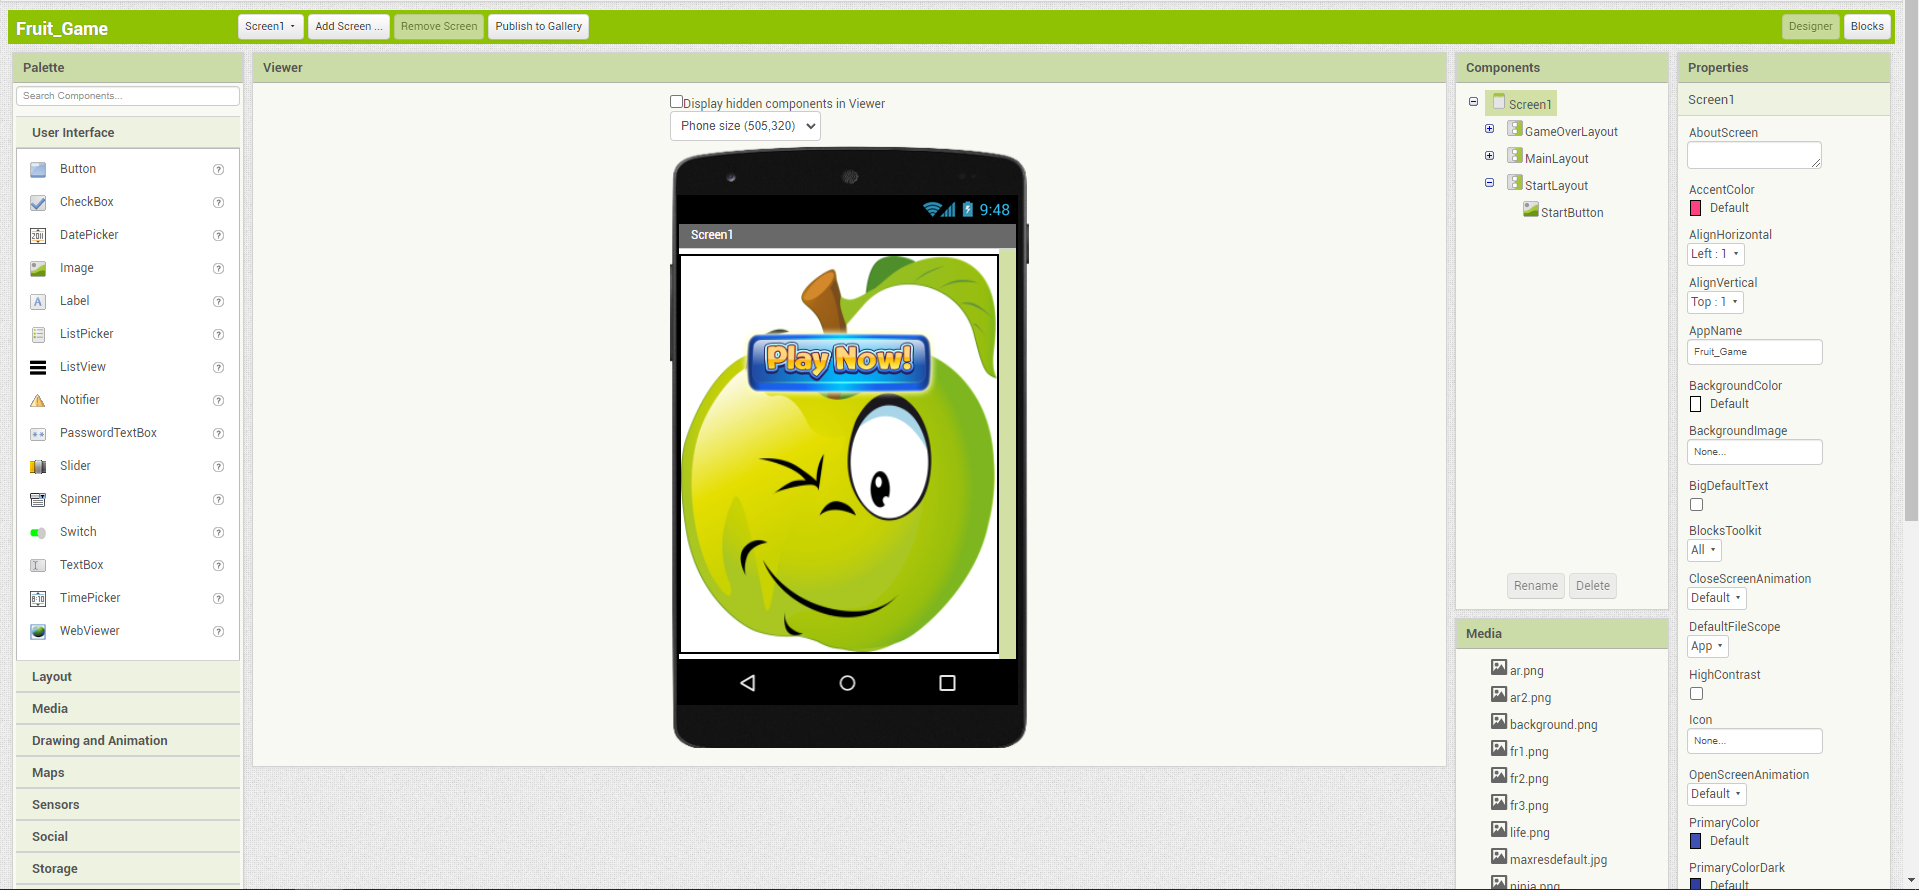
\includegraphics[width=1.0\linewidth,height=0.5\linewidth]{fig120001.png}
  \caption{Събери плодовете}
\label{fig120001}
\end{figure}

\section{Създаване на дизайна}
Конструирането на играта започва със създаването на дизайна, как ще изглежда играта. Първата стъпка е добавяне на Layout, който да бъде VerticalArrangement. Той е необходим за началния екран, когато играта започне. Размерите на този елемент трябва да бъдат такива каквито са на екрана на телефона. За това свойствата височина и ширина трябва да се сменят.

\begin{figure}[H]
  \centering
  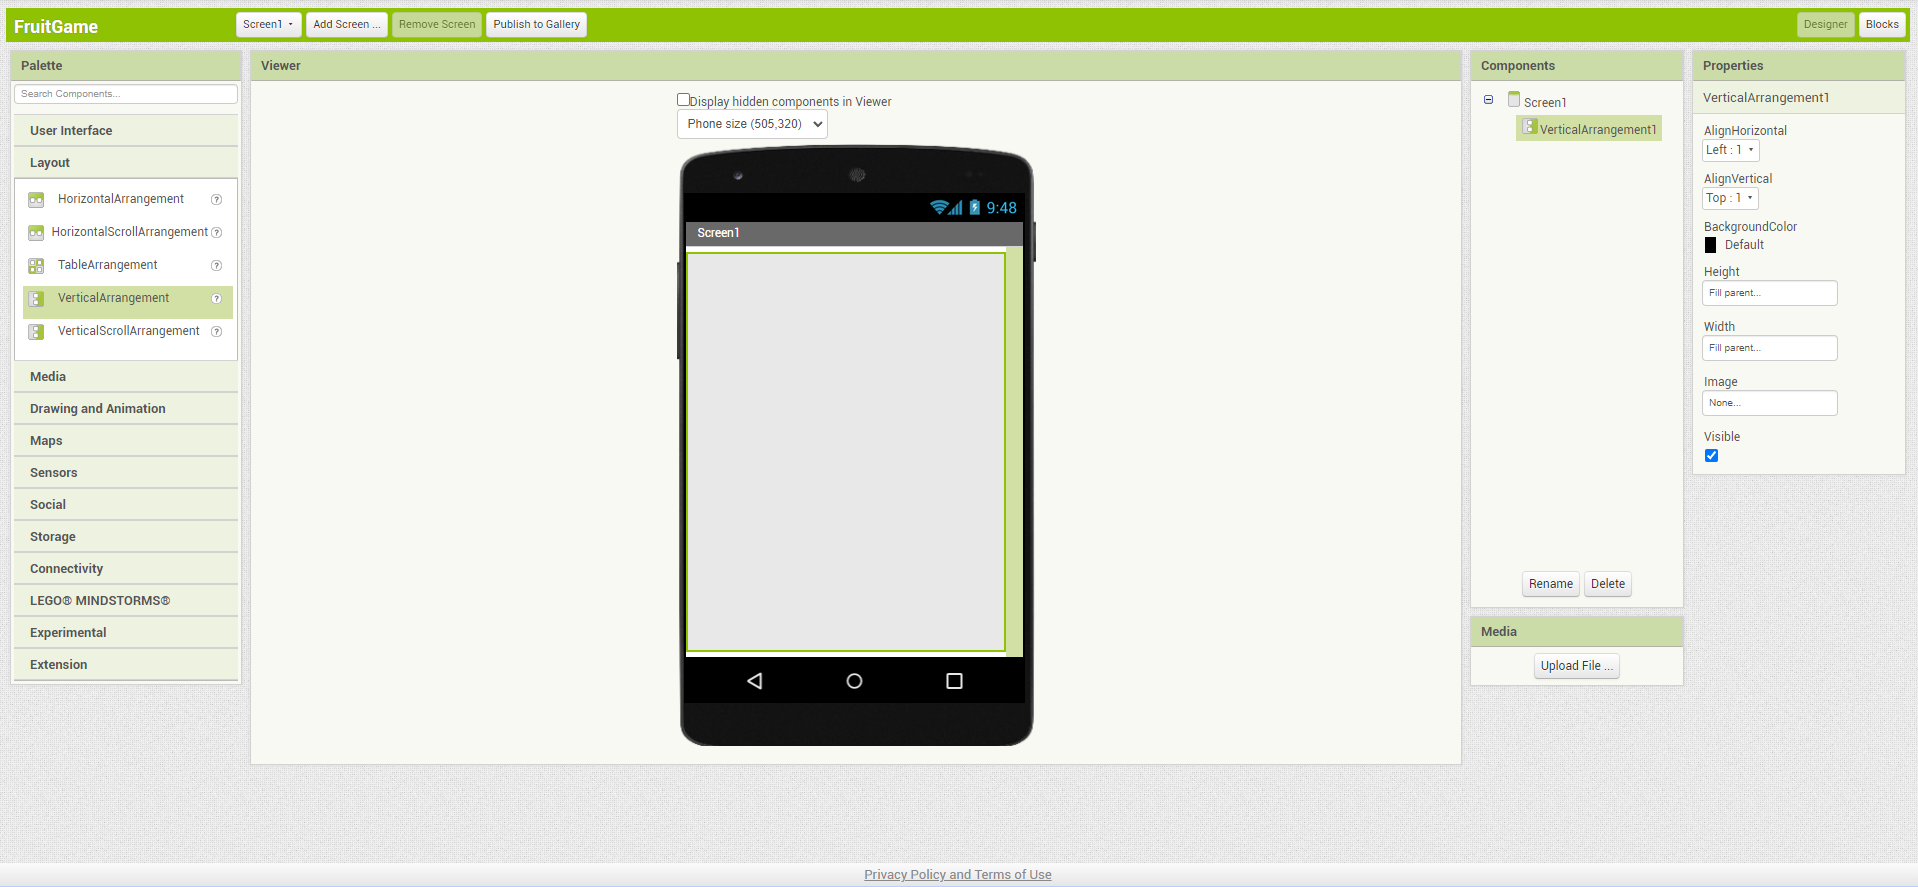
\includegraphics[width=1.0\linewidth,height=0.5\linewidth]{fig120002.png}
  \caption{Начален екран}
\label{fig120002}
\end{figure}

За да е по- атрактивно началото може да се добави изображение. Всички изображения, които са показани в този пример могат да бъдат заменени. Може да се използват всякакви изображения, които се разпространяват със свободен лиценз.

Към свойството Image трябва да се добави избраното изображение, за да се визуализира върху екрана на телефона, когато играта започне.

\begin{figure}[H]
  \centering
  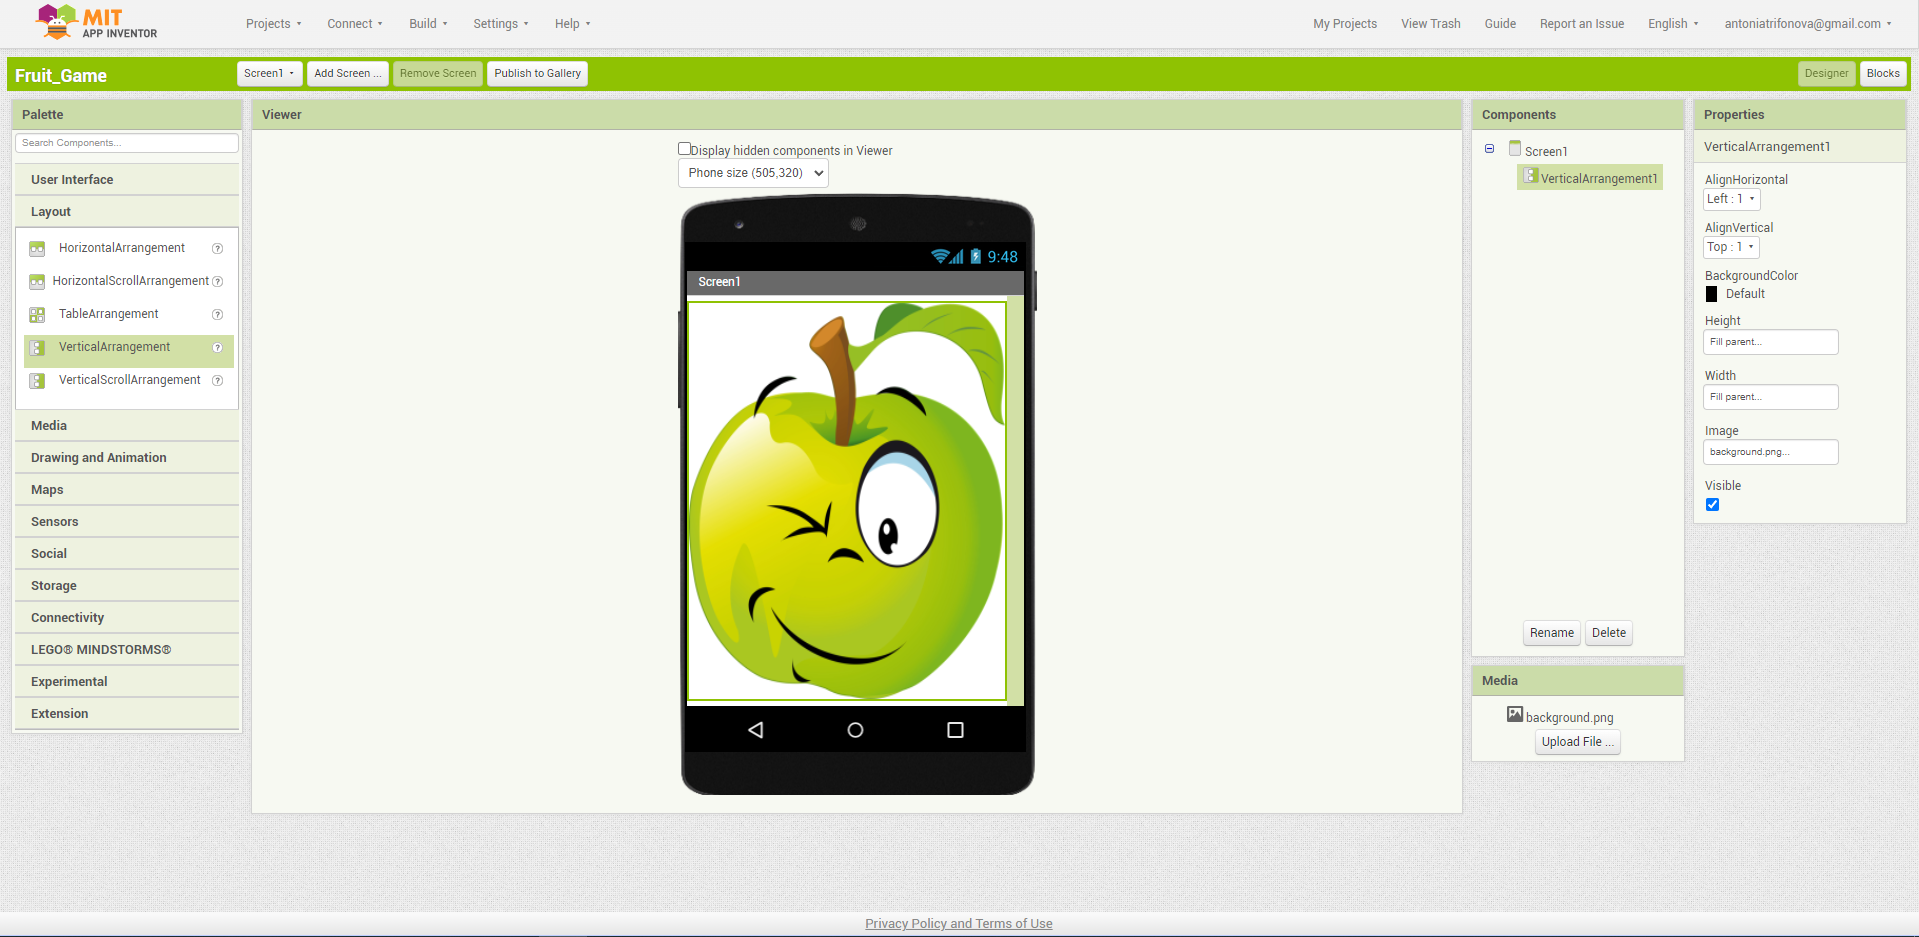
\includegraphics[width=1.0\linewidth,height=0.5\linewidth]{fig120003.png}
  \caption{Фон на началния екран}
\label{fig120003}
\end{figure}

Играта ще започне, когато играчът натисне бутона за начало. За тази цел трябва да бъде добавен и елемент за бутона. Възможно е да се използва вградения елемент за бутон, но за да се направи играта по- атрактивна може да се използва елемента Image. Може да се използва изображение за бутона. Важно е да се маркира свойството Clickable. Свойствата Height и Width отговарят за това колко да бъде високо и широко изображението.

\begin{figure}[H]
  \centering
  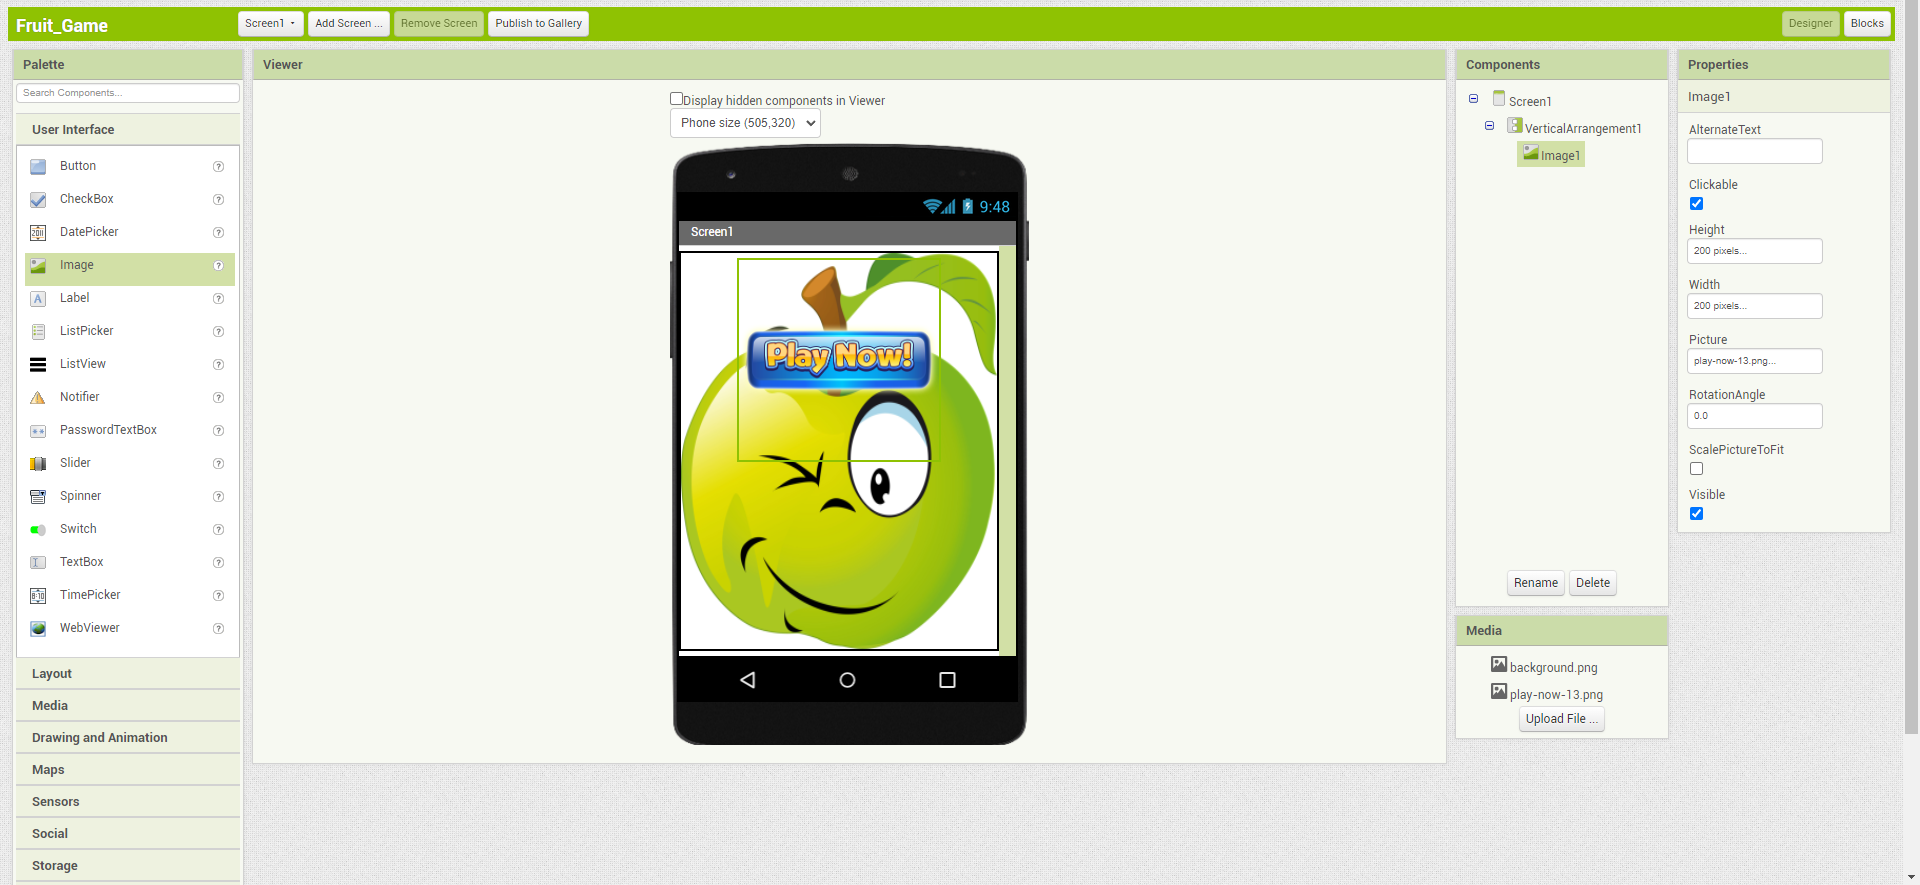
\includegraphics[width=1.0\linewidth,height=0.5\linewidth]{fig120004.png}
  \caption{Бутон за начало}
\label{fig120004}
\end{figure}

Когато играта започне ще се появява този изглед. Когато играчът натисне бутонът трябва да се появи друг изглед, в който ще се появи героят, който ще бъде управляван и падащите плодове. С цел да се различават различните изгледи на играта, когато се програмират е добра практика да имат описателни имена. Елементът VerticalArrangement1 ще се казва StartLayout, а елементът Image1 ще се казва StartButton.

\begin{figure}[H]
  \centering
  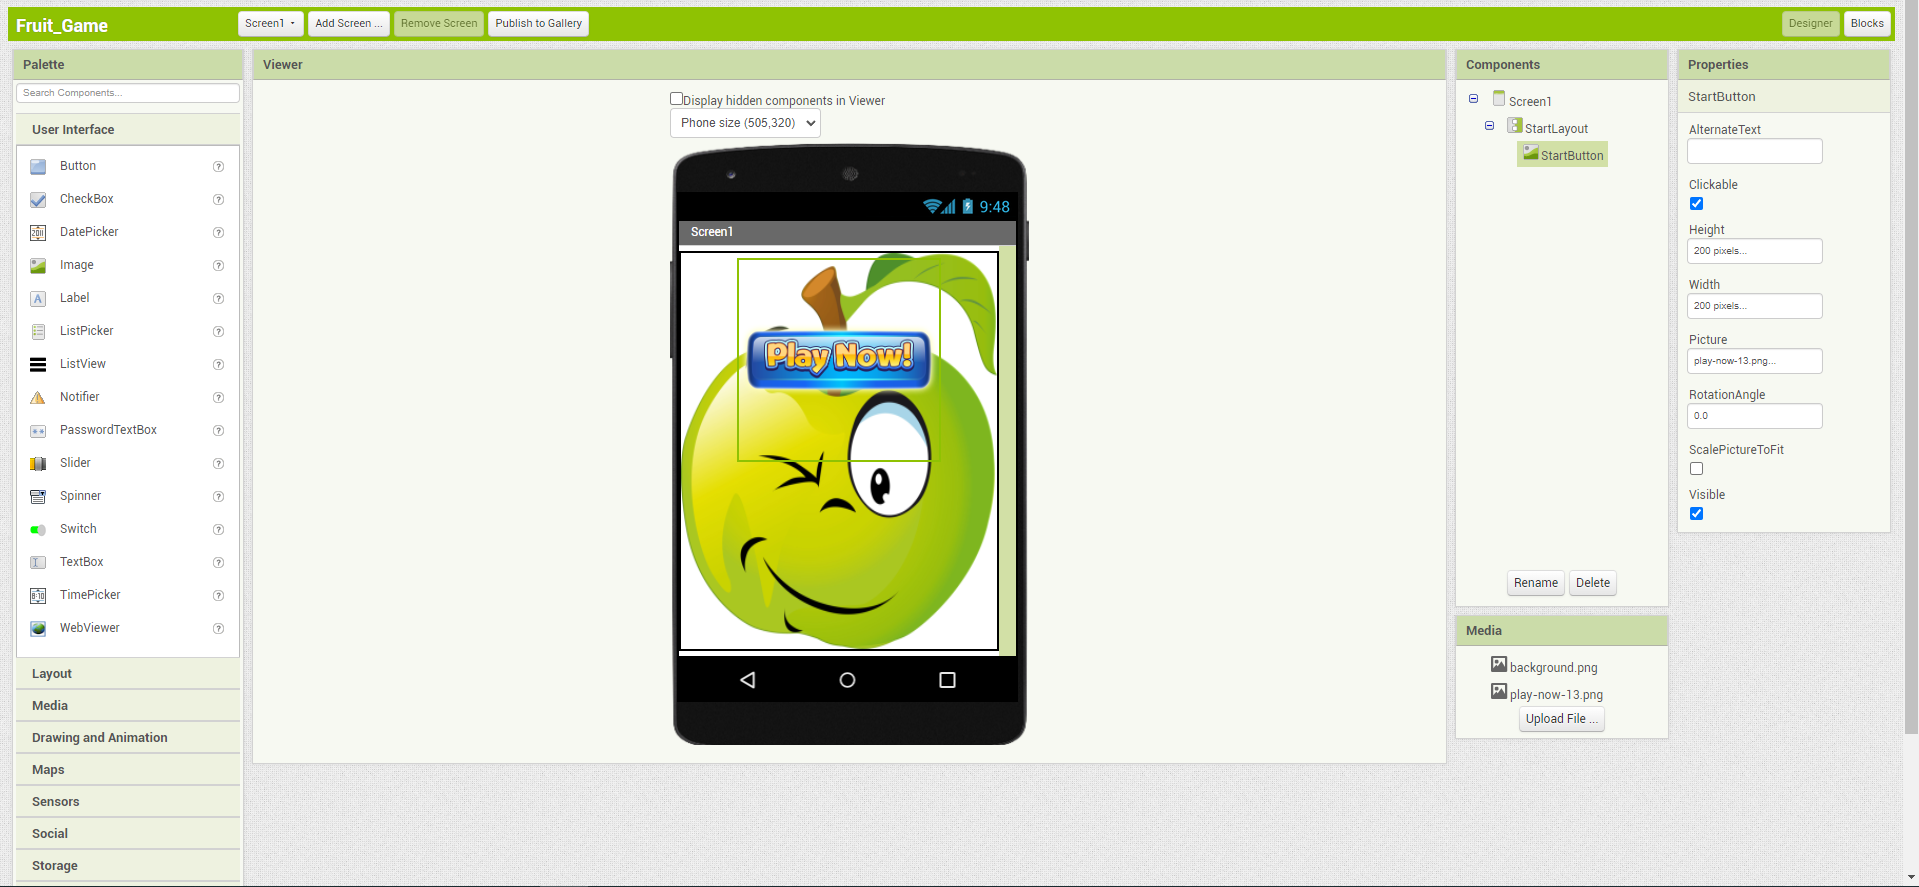
\includegraphics[width=1.0\linewidth,height=0.5\linewidth]{fig120005.png}
  \caption{Финална версия на началния екран}
\label{fig120005}
\end{figure}

За създаването на другия изглед отново трябва да се добави елемент VerticalArrangement, който да се казва MainLayout. Височината и ширината на този елемент трябва да бъдат същите, каквито са на екрана. С цел да се направи по- лесно дизайна на този изглед трябва да се размаркира свойството Visible на елемента StartLayout.

\begin{figure}[H]
  \centering
  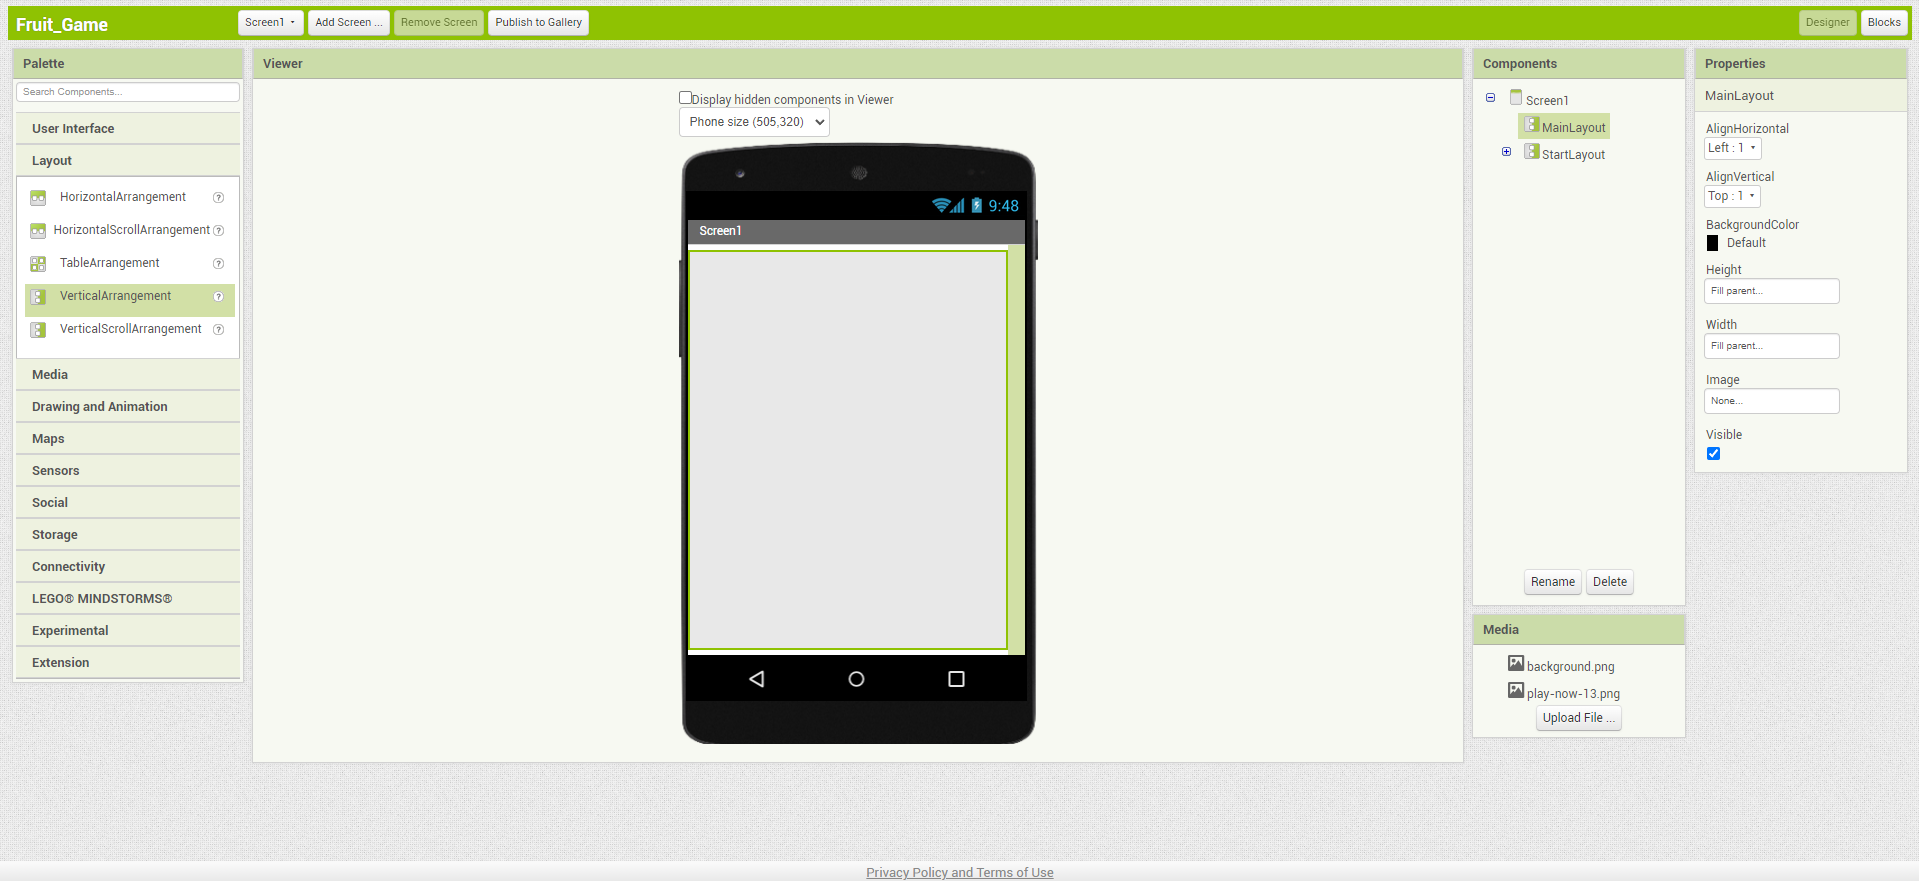
\includegraphics[width=1.0\linewidth,height=0.5\linewidth]{fig120006.png}
  \caption{Създаване на основен екран на играта}
\label{fig120006}
\end{figure}

Към елемента MainLayout следва да се добавят елементите Canvas и HorizontalArrangement.
Елементът Canvas е необходим, защото той позволява на елементите, които са вътре в него да се движат. В играта съществуват няколко елемента, които ще се движат. От една страна това е героят, който ще улавя плодовете, а от друга самите плодове.
Височината и ширината на този елемент трябва да бъдат същите, каквито са на екрана. Отново може да бъде добавен и фон на този елемент.

\begin{figure}[H]
  \centering
  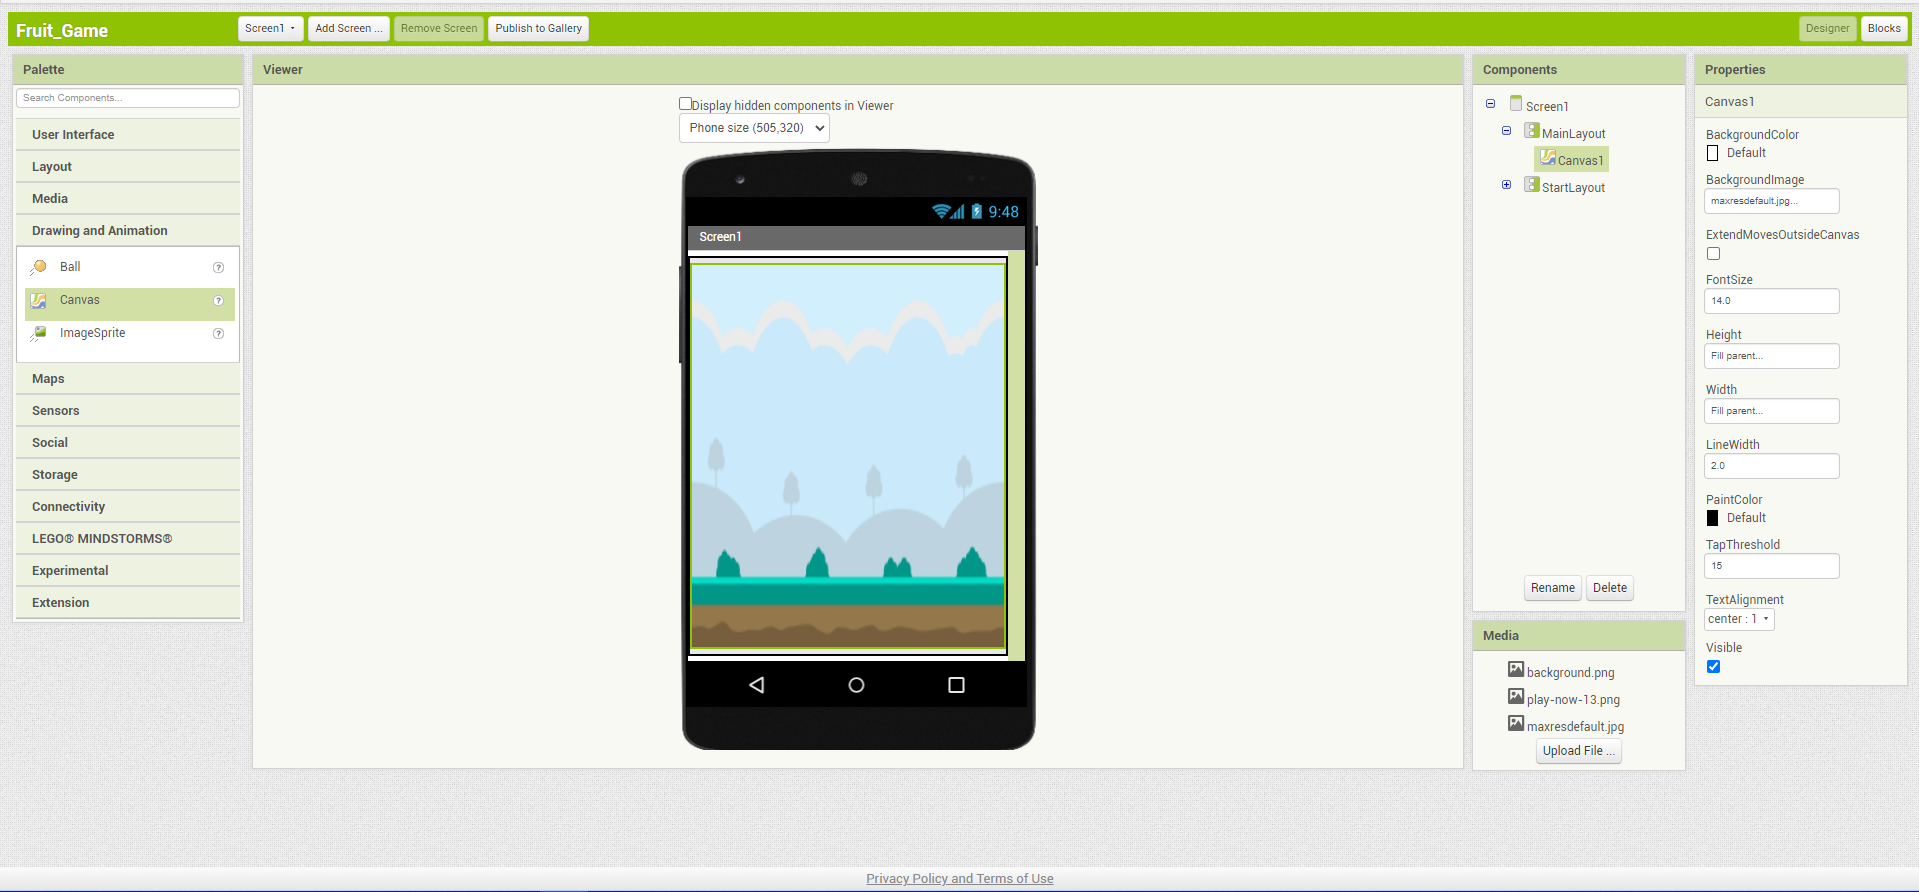
\includegraphics[width=1.0\linewidth,height=0.5\linewidth]{fig120007.png}
  \caption{Добавяне на фон към основния екран на играта}
\label{fig120007}
\end{figure}

Към този елемент трябва да бъдат добавени няколко изображения на плодове. Също така изображение, което да е героят и три изображения, които да са неговите животи. С промяната на свойствата Height и Width може да се променят размерите им, а чрез промяна на свойствата X, Y и Z може да се промени и тяхното положение. Важно е да се променят и имената на елементите, за да може да се разпознават, когато се премине към програмирането им.
На фигурата е показано примерно разположение на плодовете, героя и неговите животи. За целите на играта не е от значение броя на плодовете или тяхното разположение.

\begin{figure}[H]
  \centering
  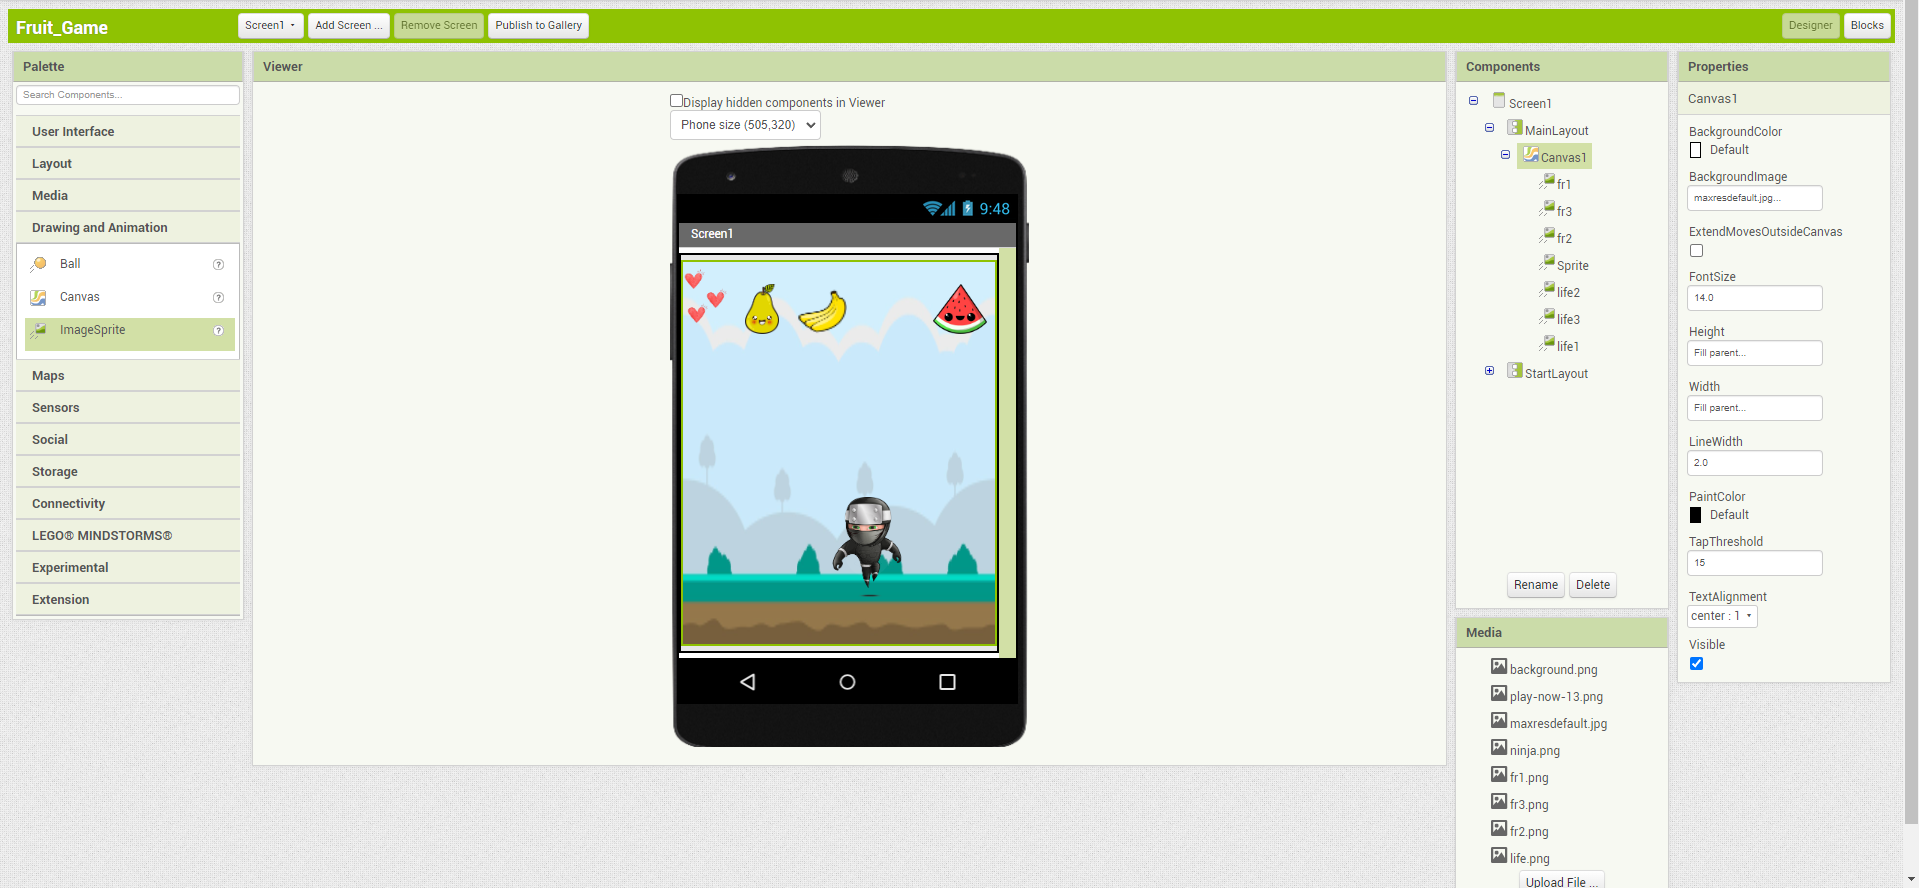
\includegraphics[width=1.0\linewidth,height=0.5\linewidth]{fig120008.png}
  \caption{Добавяне на плодовете, животите и героя към играта}
\label{fig120008}
\end{figure}

За да бъде завършен този изглед трябва да се добави елемент HorizontalArrangement, към който ще се добавят двата бутона - стрелка наляво и стрелка надясно. Тези бутони ще контролират играча да се движи. Между тях може да бъде поставен и елемент Label, в който ще се показва колко точки е спечелил играчът.
Ширината на елемента HorizontalArrangement трябва да бъде колкото е тази на екрана. Височината му трябва да бъде малка, например 10 процента. За да могат елементите вътре да се подредят трябва да се променят свойствата AlignHorizontal и AlignVertical да бъдат със стойност Center.

\begin{figure}[H]
  \centering
  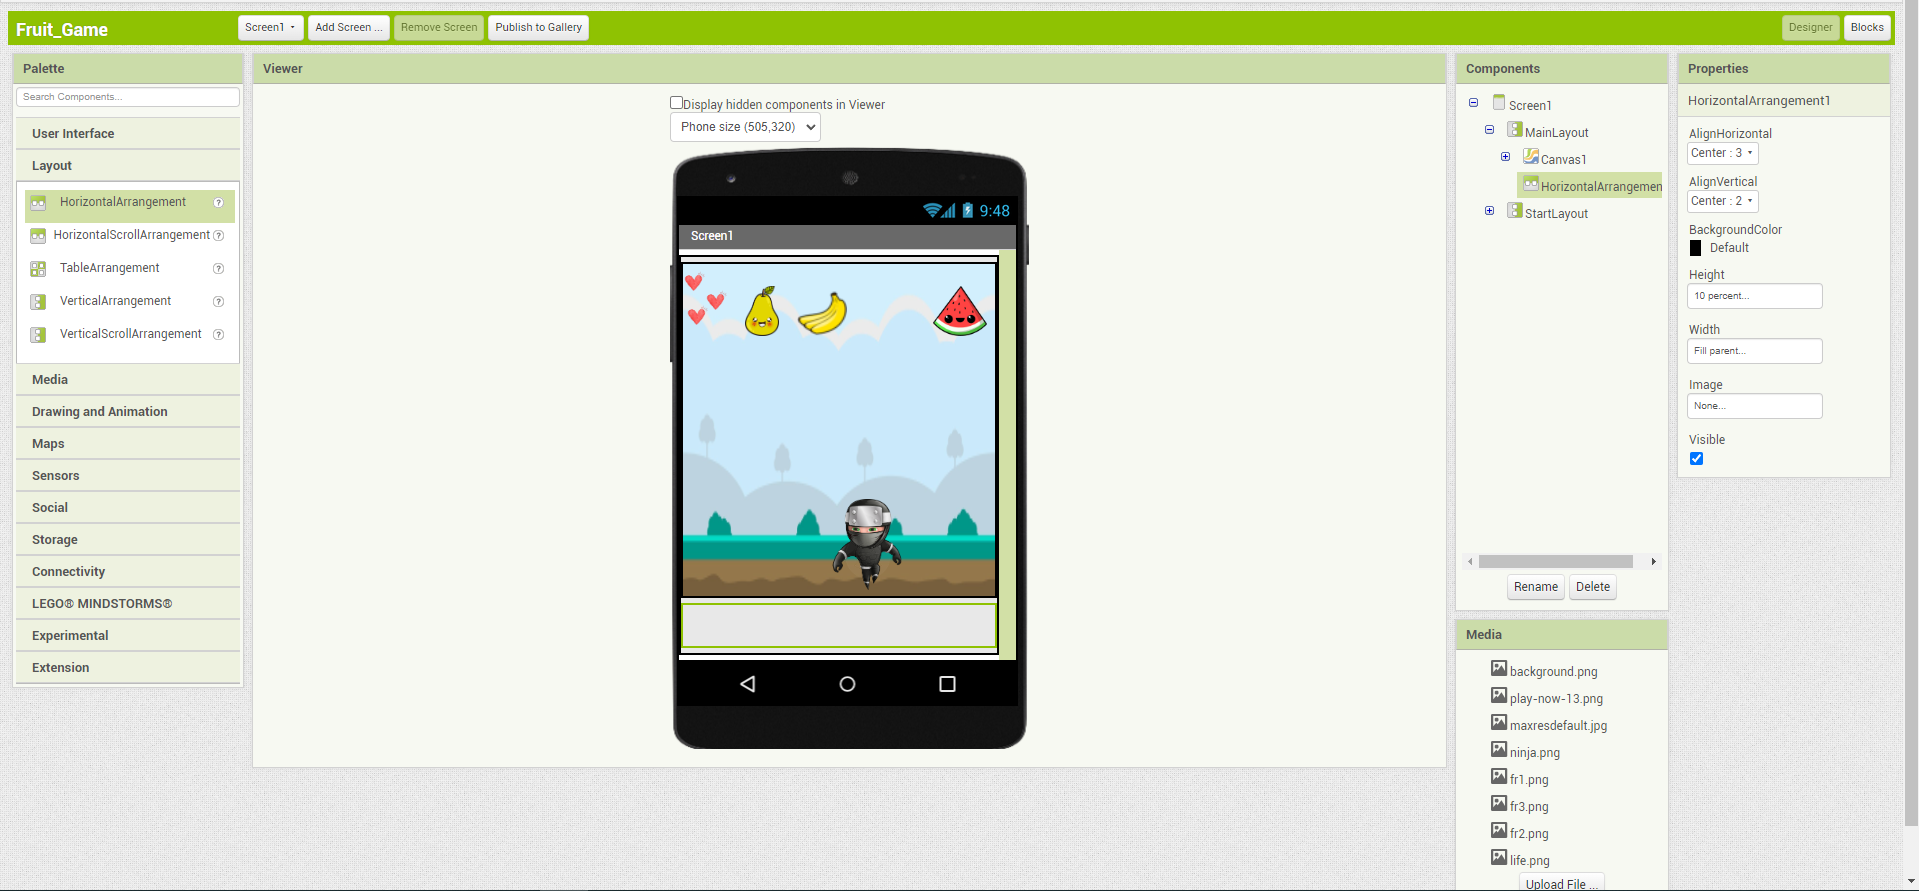
\includegraphics[width=1.0\linewidth,height=0.5\linewidth]{fig120009.png}
  \caption{Добавяне на лента за контролите}
\label{fig120009}
\end{figure}

Следва да бъдат добавени бутоните, като се променят техните размери и се добавят изображения, така че да заприличат на стрелки лява и дясна. 

\begin{figure}[H]
  \centering
  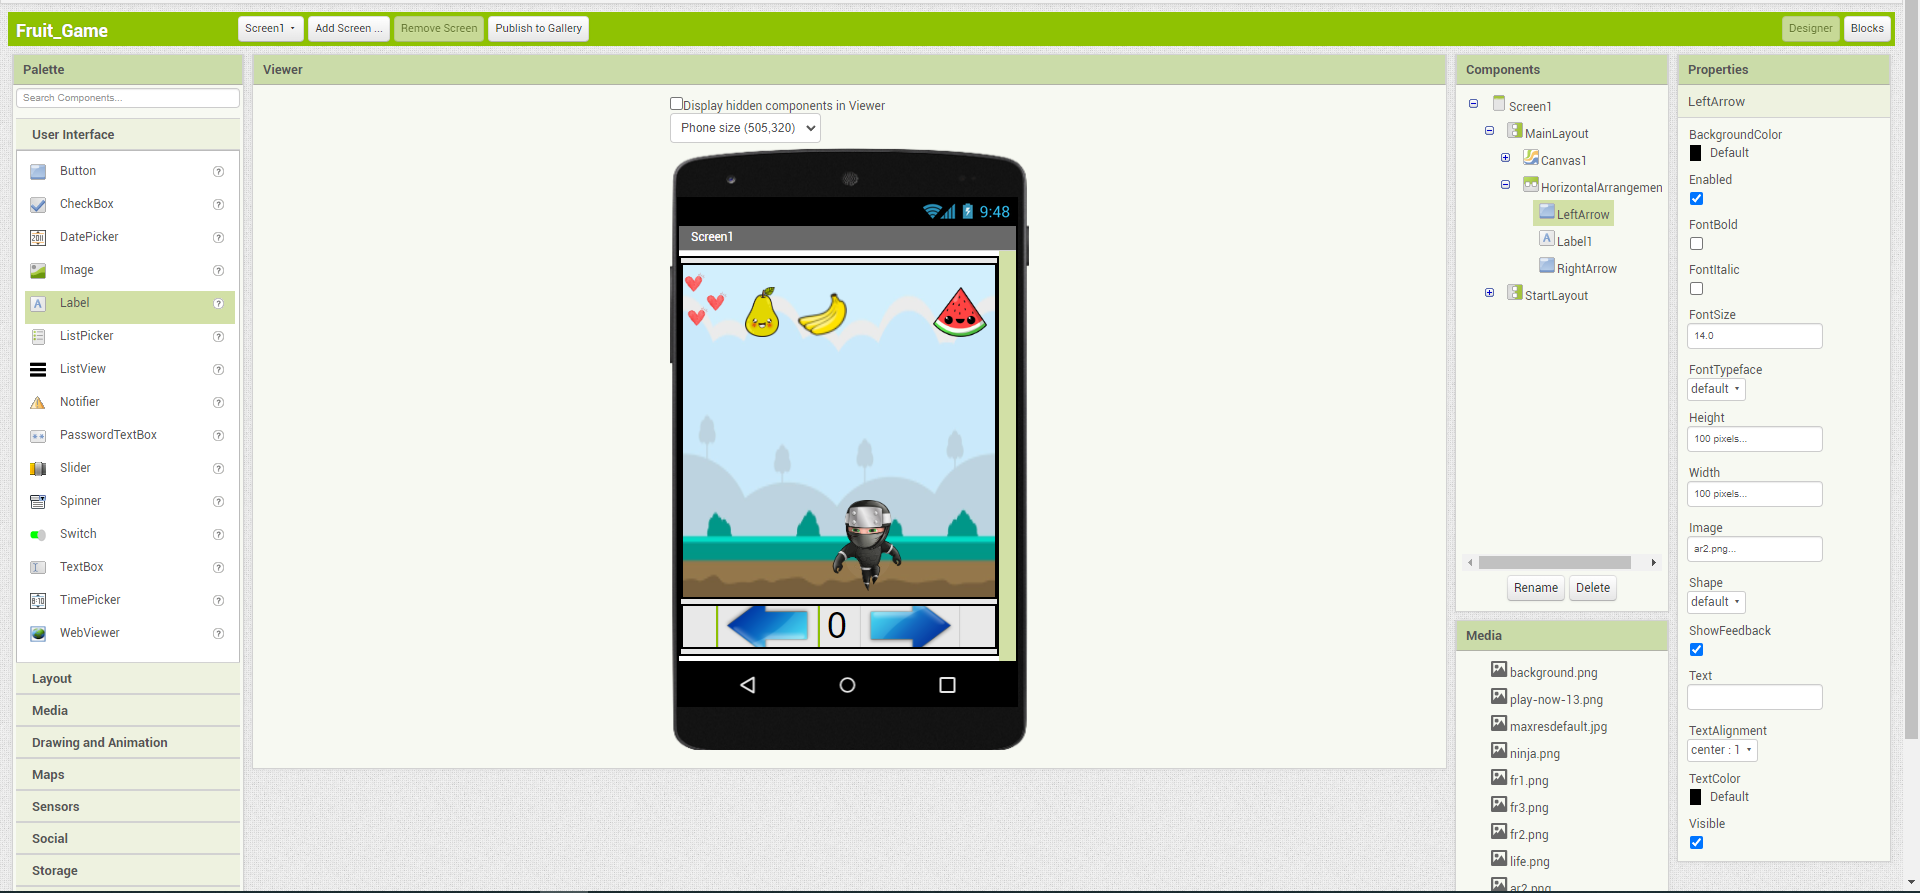
\includegraphics[width=1.0\linewidth,height=0.5\linewidth]{fig120010.png}
  \caption{Добавяне на контролите}
\label{fig120010}
\end{figure}

За елемента Label, където ще се изписват точките трябва да се промени стойността на свойството FontSize, за да може текста да бъде по- голям и да се вижда.

\begin{figure}[H]
  \centering
  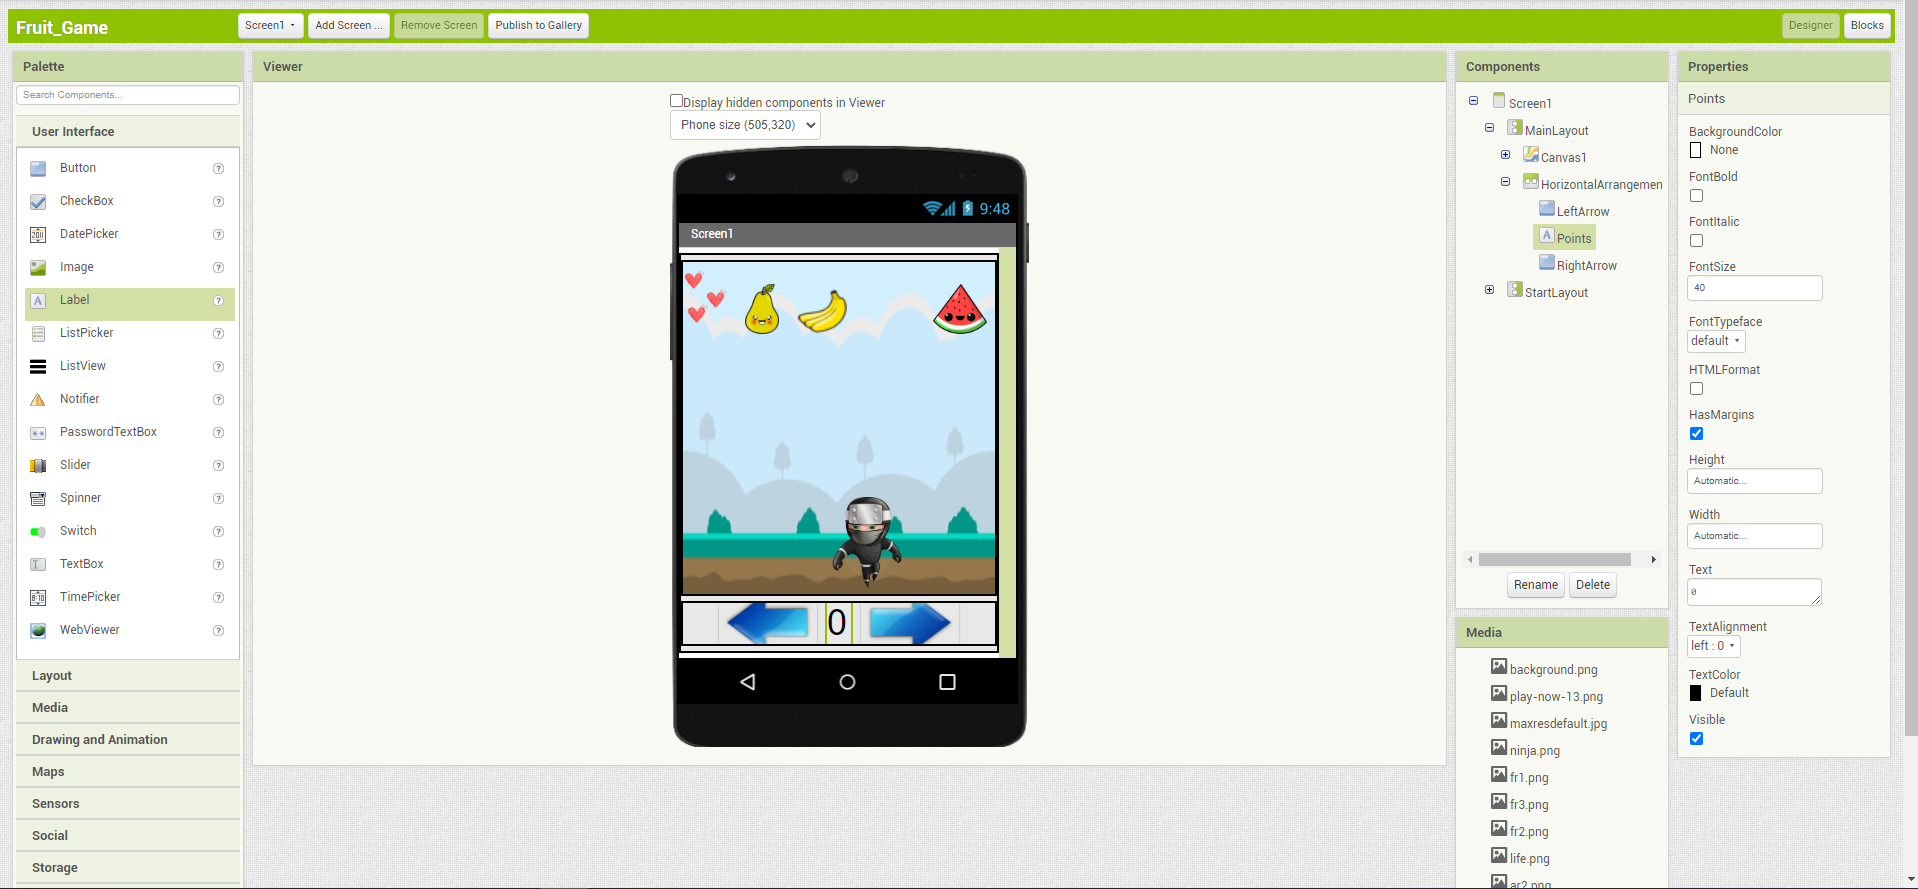
\includegraphics[width=1.0\linewidth,height=0.5\linewidth]{fig120011.png}
  \caption{Промяна на размера на точките}
\label{fig120011}
\end{figure}

Последният изглед, на който трябва да бъде направен дизайн е когато играчът загуби животите си. Тогава следва да се покаже бутон “Опитай пак”. За да може по- лесно да се направи дизайна трябва да се размаркира свойството Visible на елемента MainLayout.

\begin{figure}[H]
  \centering
  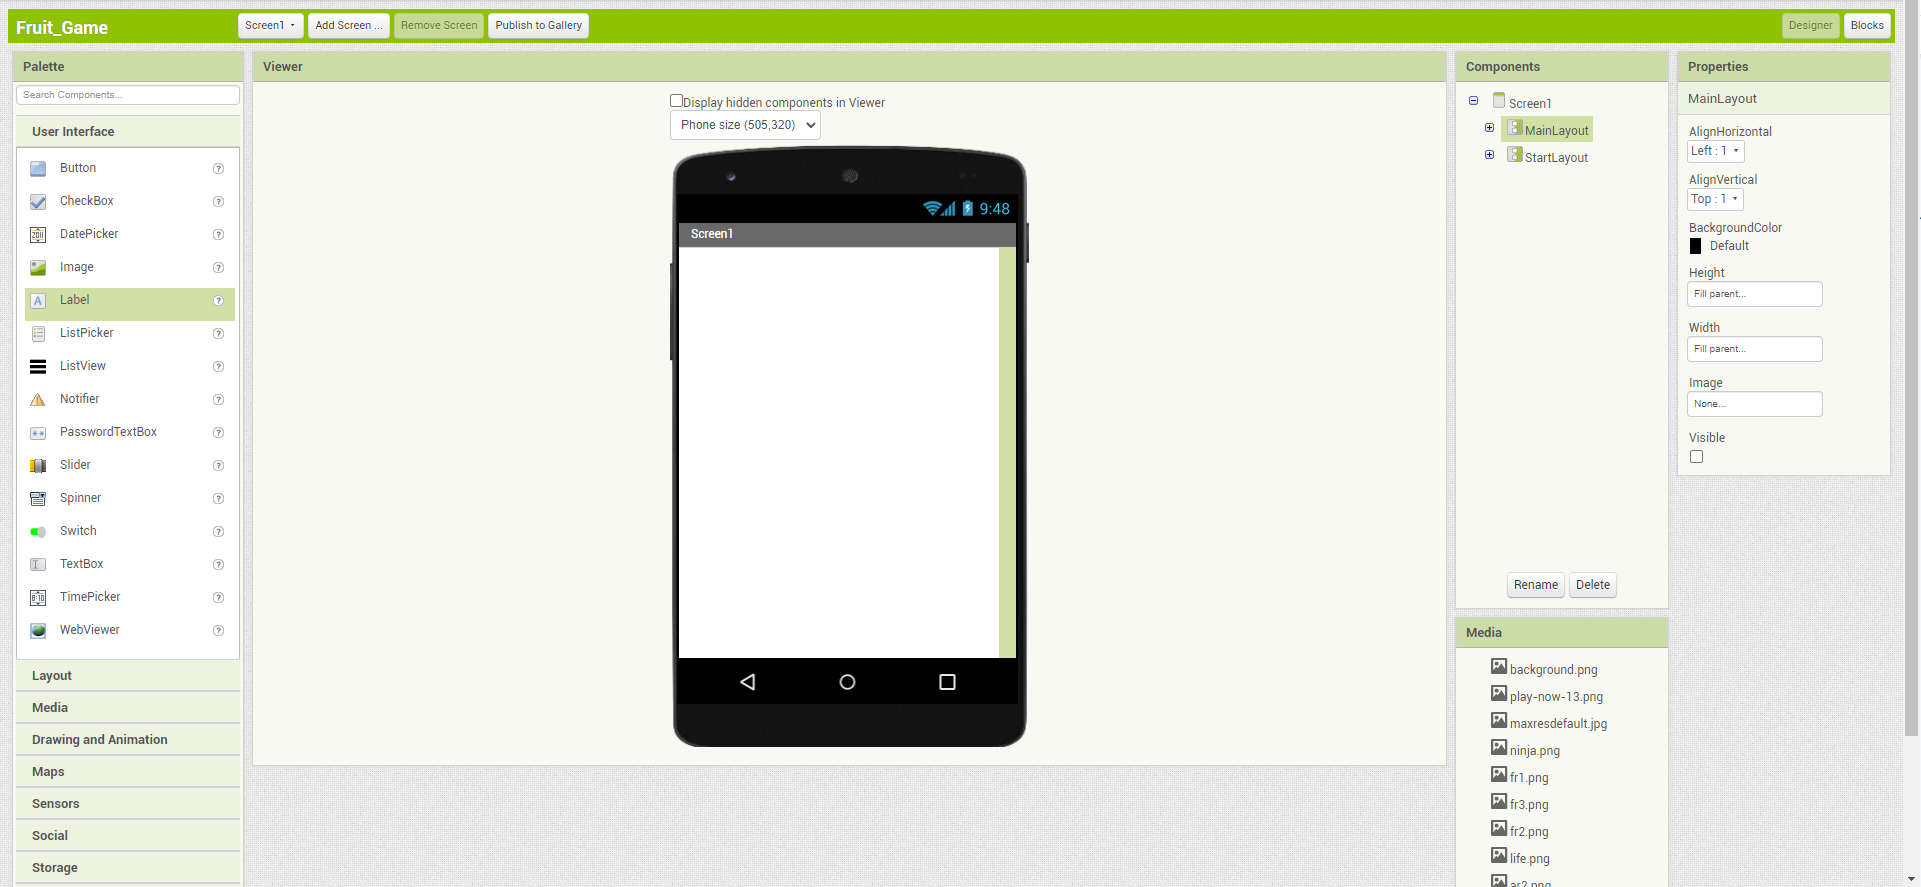
\includegraphics[width=1.0\linewidth,height=0.5\linewidth]{fig120012.png}
  \caption{Добавяне на изглед за край на играта}
\label{fig120012}
\end{figure}

Изгледът, който е ще е за край на играта трябва да бъде отново HorizontalArrangement, като размерите височина и ширина трябва да бъдат същите, каквито са на екрана. Може да се промени цвета на фона на този елемент или да се добави картинка за край на играта. Стойностите на свойствата AlignHorizontal и AlignVertical трябва да бъдат със стойност Center, за да може бутона за рестартиране на играта да бъде поставен в средата.

\begin{figure}[H]
  \centering
  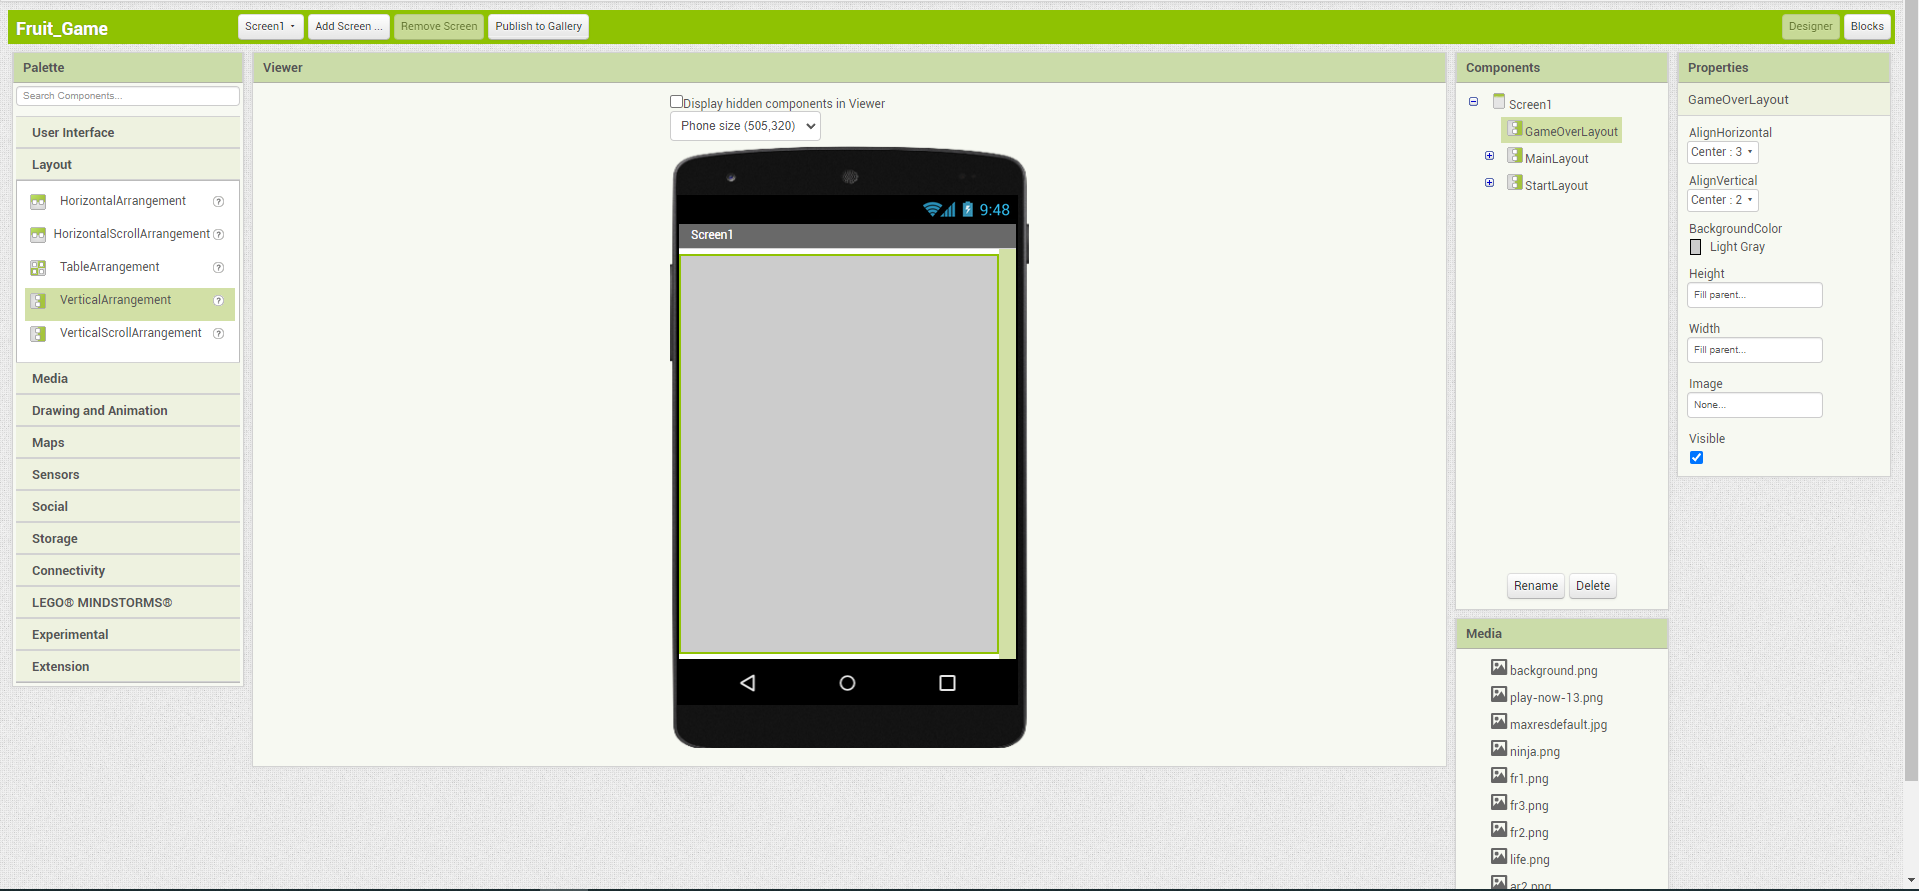
\includegraphics[width=1.0\linewidth,height=0.5\linewidth]{fig120013.png}
  \caption{Промяна на цвета на фона}
\label{fig120013}
\end{figure}

Последно трябва да бъде добавен и бутона за рестартиране на играта. Свойствата за формата, големината на текста и цвета на бутона могат да бъдат променени.

\begin{figure}[H]
  \centering
  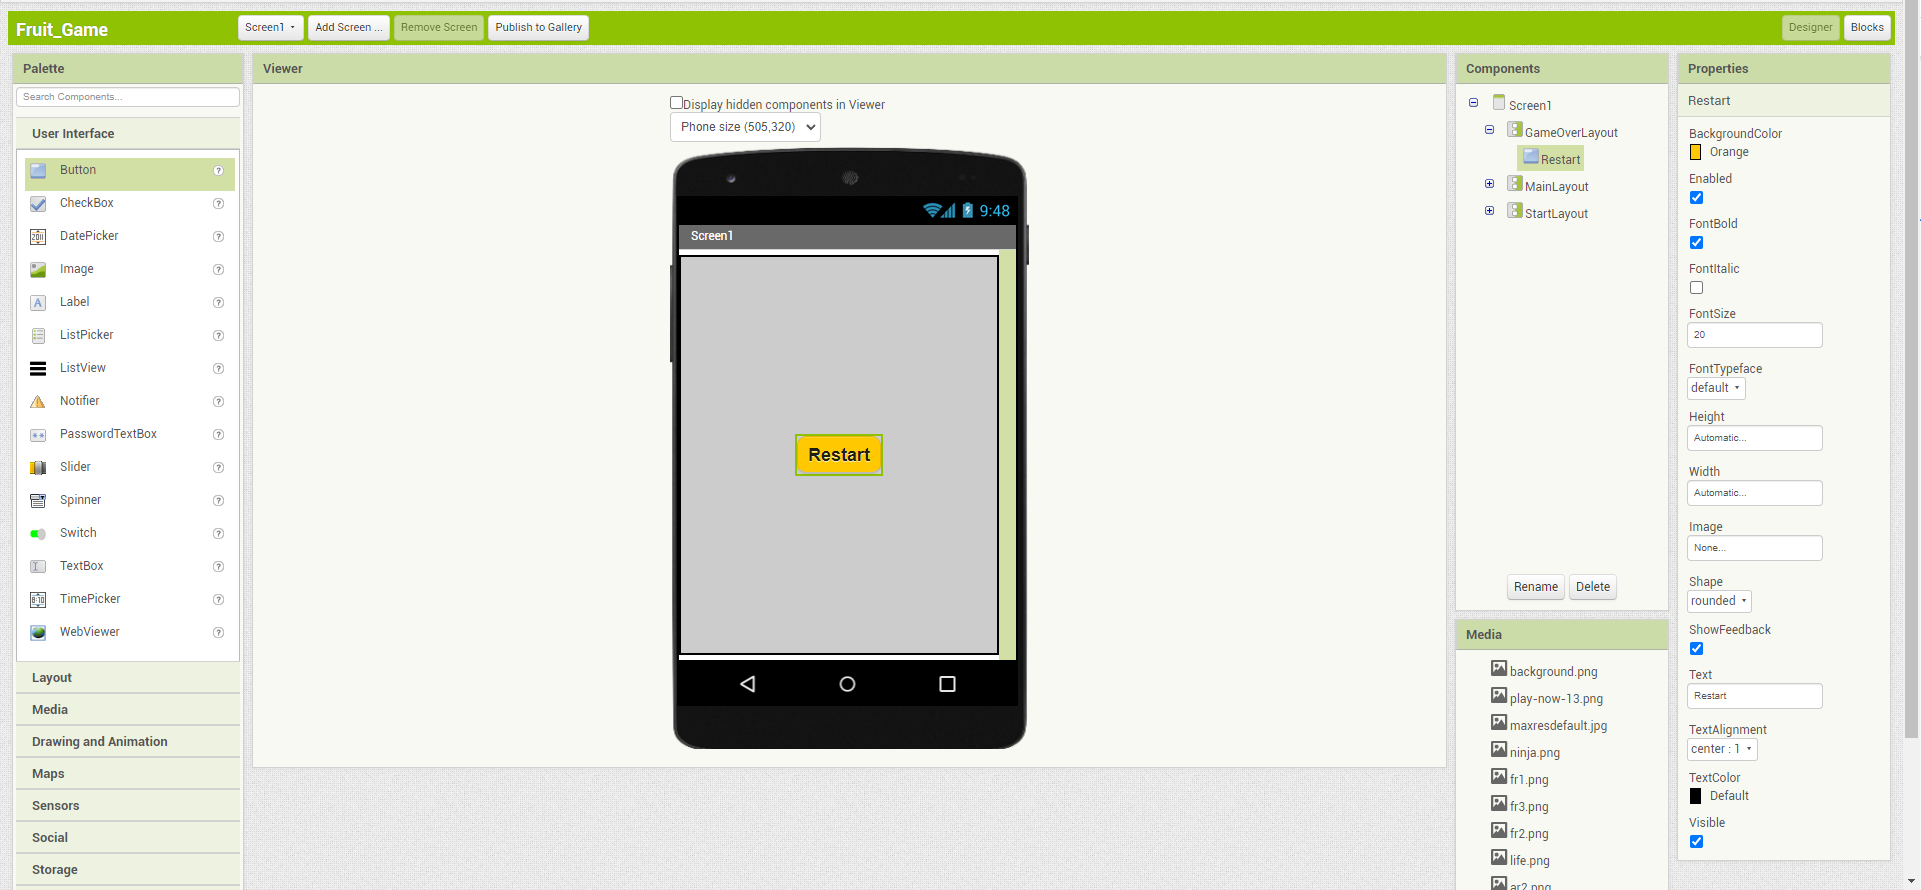
\includegraphics[width=1.0\linewidth,height=0.5\linewidth]{fig120014.png}
  \caption{Добавяне на бутон за рестарт на играта}
\label{fig120014}
\end{figure}

Свойството Visible на елемента GameOverLayout трябва да бъде размаркирано. Единствено екрана за начало на играта трябва да се вижда. За това трябва да се маркира за елемента StartLayout.

\begin{figure}[H]
  \centering
  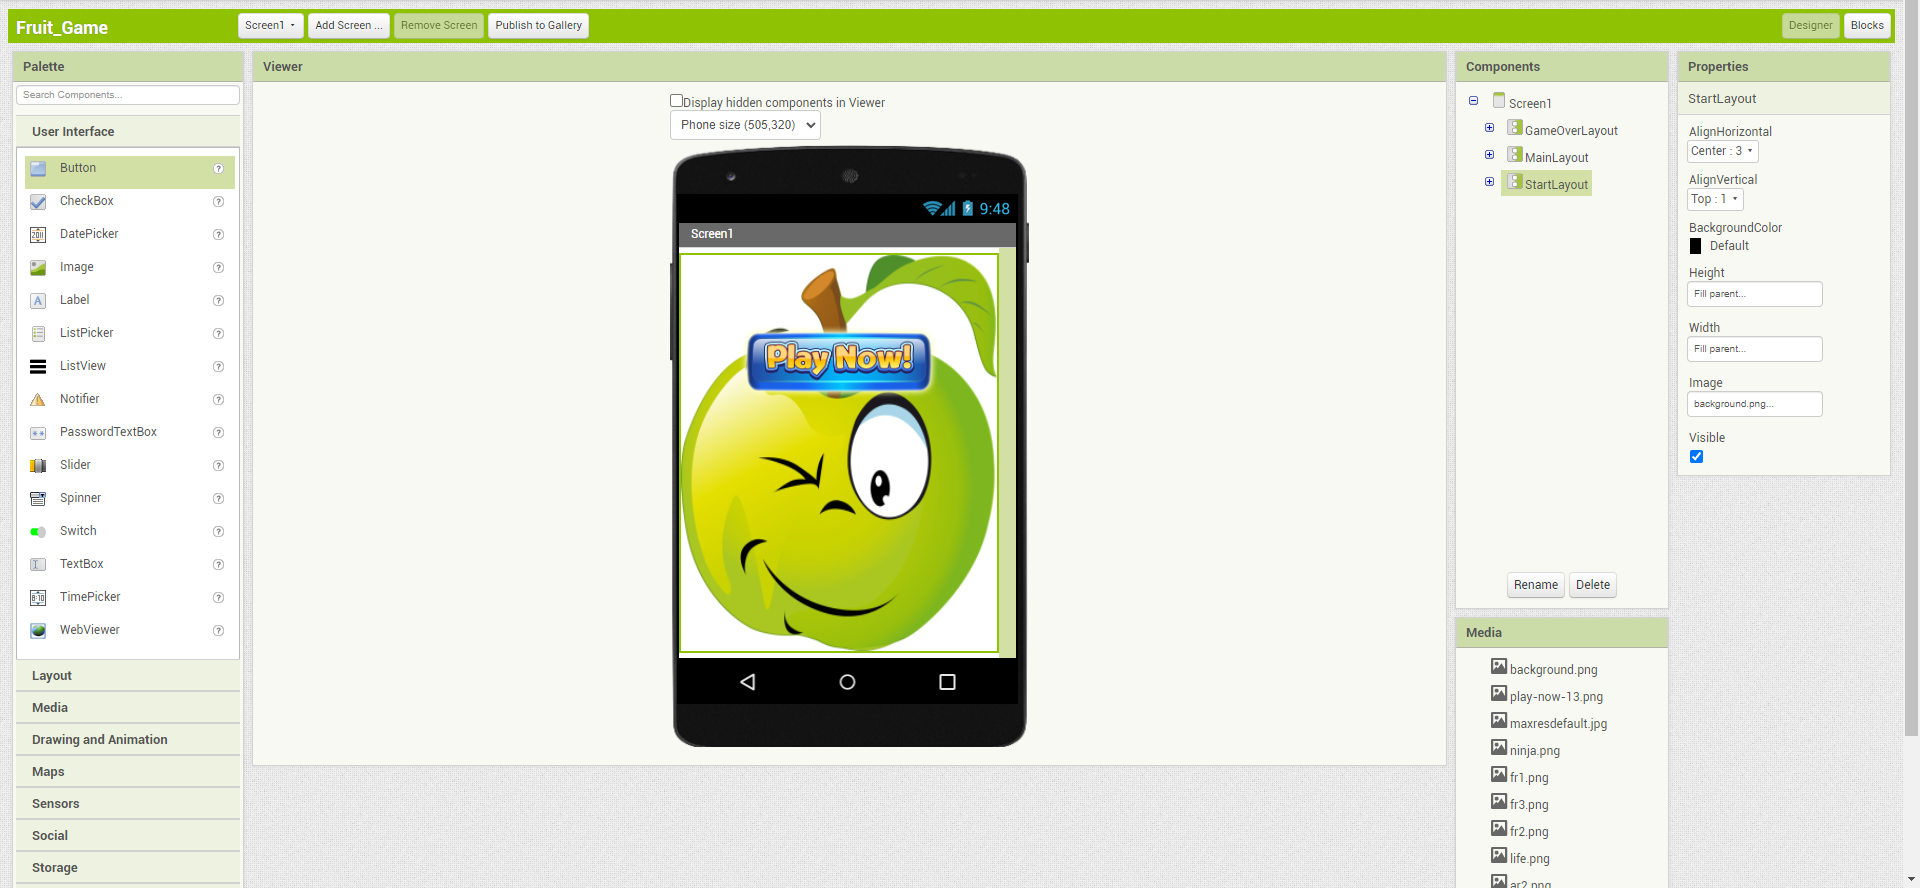
\includegraphics[width=1.0\linewidth,height=0.5\linewidth]{fig120015.png}
  \caption{Маркиране на свойството Visible за началния екран}
\label{fig120015}
\end{figure}

\section{Създаване на програмата}
В конструирането на кода на играта ще бъдат използвани блокове, които се наричат “процедури”. Процедурата се характеризира с име и набор от инструкции. Те се изпълняват тогава, когато тя бъде извикана. Целта на процедурата е да съдържа инструкции, които се повтарят в даден момент в кода. В следващите стъпки е обяснено къде и защо има нужда да се използват процедури.

Първата процедура, която трябва да се създаде е за начало на играта. Инструкциите, които ще бъдат в нея са за първоначалните позиции на плодовете и задаване на скоростите, с които ще се движат. Тази последователност от стъпки трябва да се изпълни, когато играта започне, т.е. играчът натисне бутона за начало на играта, но също така и когато играчът натисне бутона за рестартиране на играта. За това се използва процедура с цел избягването на конструиране на едни и същи стъпки два пъти.

\begin{figure}[H]
  \centering
  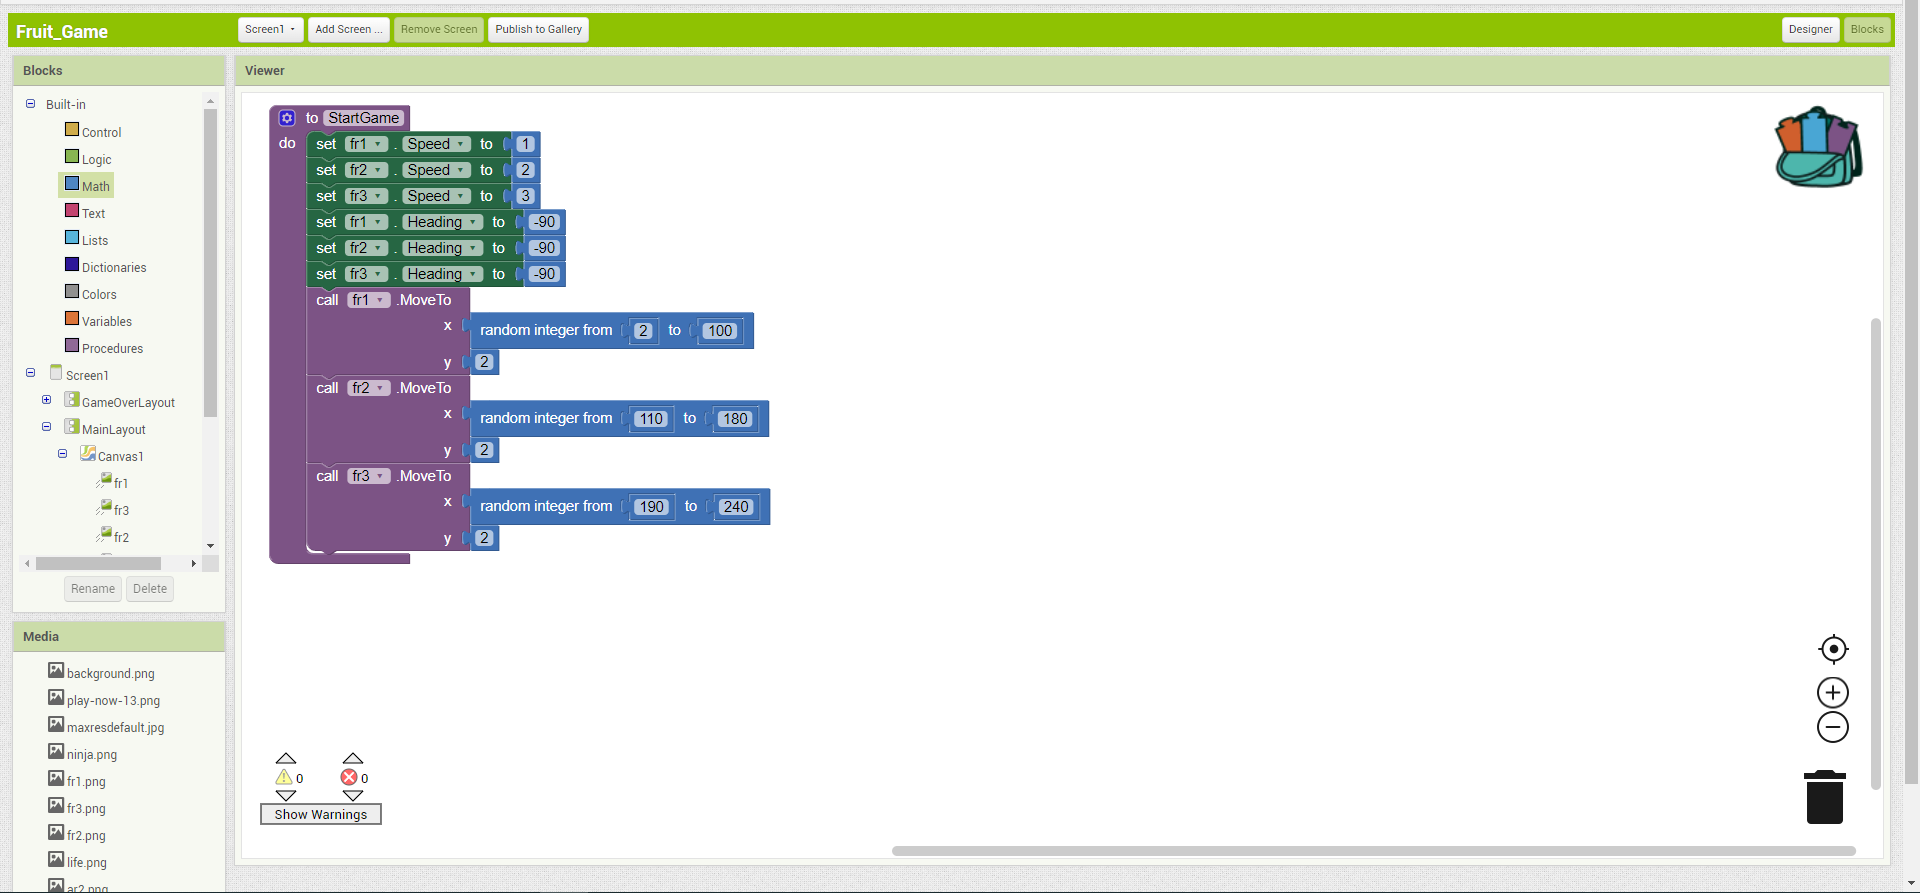
\includegraphics[width=1.0\linewidth,height=0.5\linewidth]{fig120016.png}
  \caption{Създаване на процедура за начало на играта}
\label{fig120016}
\end{figure}

Първият път когато ще се извика тази процедура е когато се натисне бутона StartButton. Освен извикването на процедурата, другите инструкции, които трябва да се изпълнят са стартовия изгледа да се скрие и да се появи основния изглед. Това се реализира с помощта на свойството Visible, което може да се контролира освен през дизайна, а и програмно.

\begin{figure}[H]
  \centering
  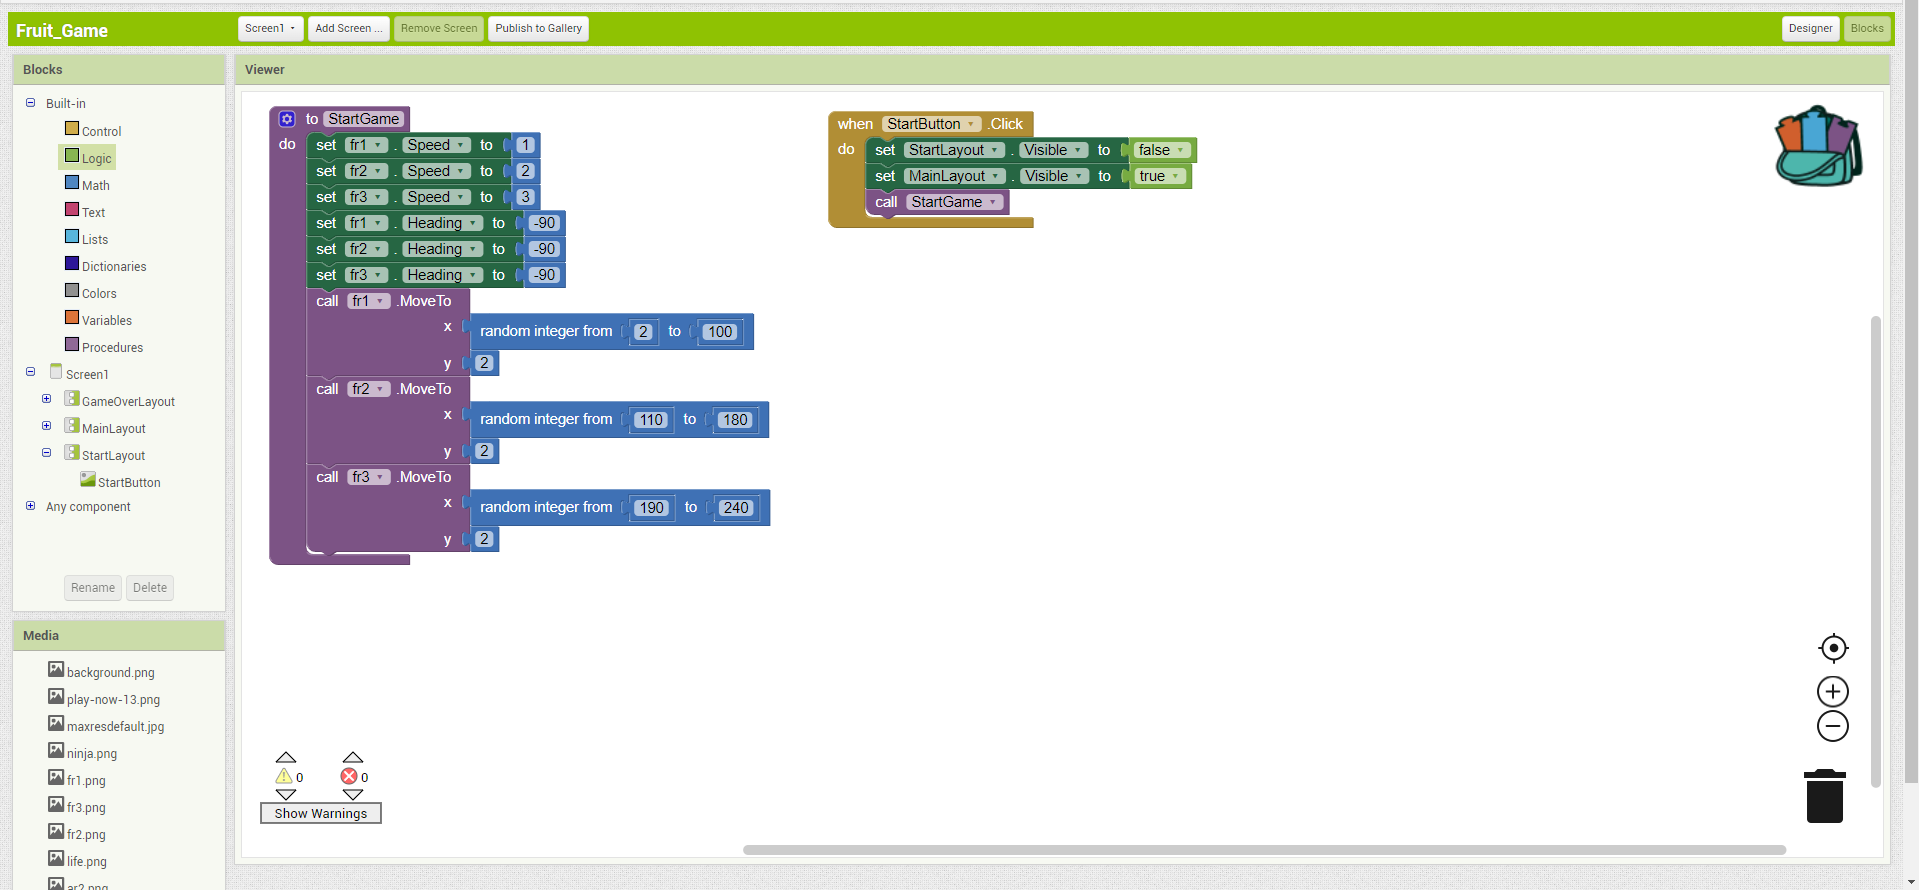
\includegraphics[width=1.0\linewidth,height=0.5\linewidth]{fig120017.png}
  \caption{Програмиране на бутона за начало на играта}
\label{fig120017}
\end{figure}

Героят на играта ще се движи наляво и надясно, когато се клика върху стрелка наляво или стрелка надясно съответно. За тази цел трябва да бъдат добавени две събития - когато се кликне върху стрелка наляво или когато се кликне върху стрелка надясно. Инструкциите в тези две събития са подобни - героят трябва да си смени позицията спрямо X координатата. В единия случай трябва да се увеличи, а в другия да се намали.

\begin{figure}[H]
  \centering
  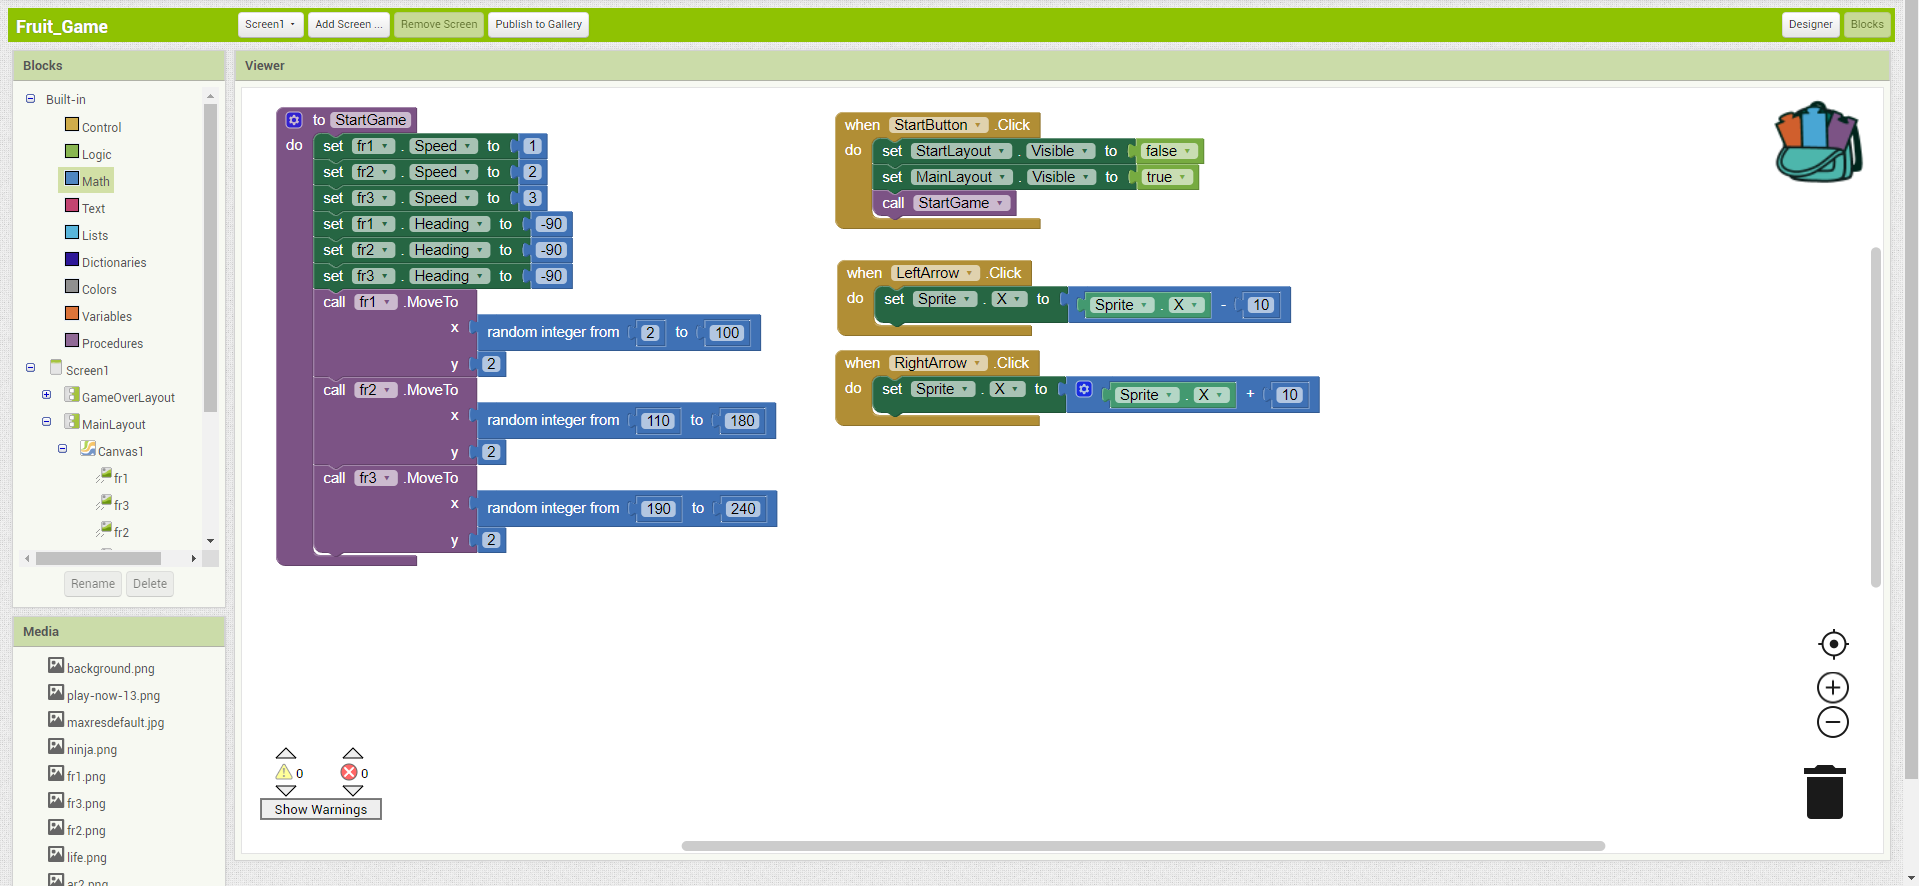
\includegraphics[width=1.0\linewidth,height=0.5\linewidth]{fig120018.png}
  \caption{Програмиране на героя да се движи}
\label{fig120018}
\end{figure}

В тази игра трябва да се създадат следните променливи - 3, които ще отговарят за скоростта на трите плода и една, която ще бъде за животите на героя.

\begin{figure}[H]
  \centering
  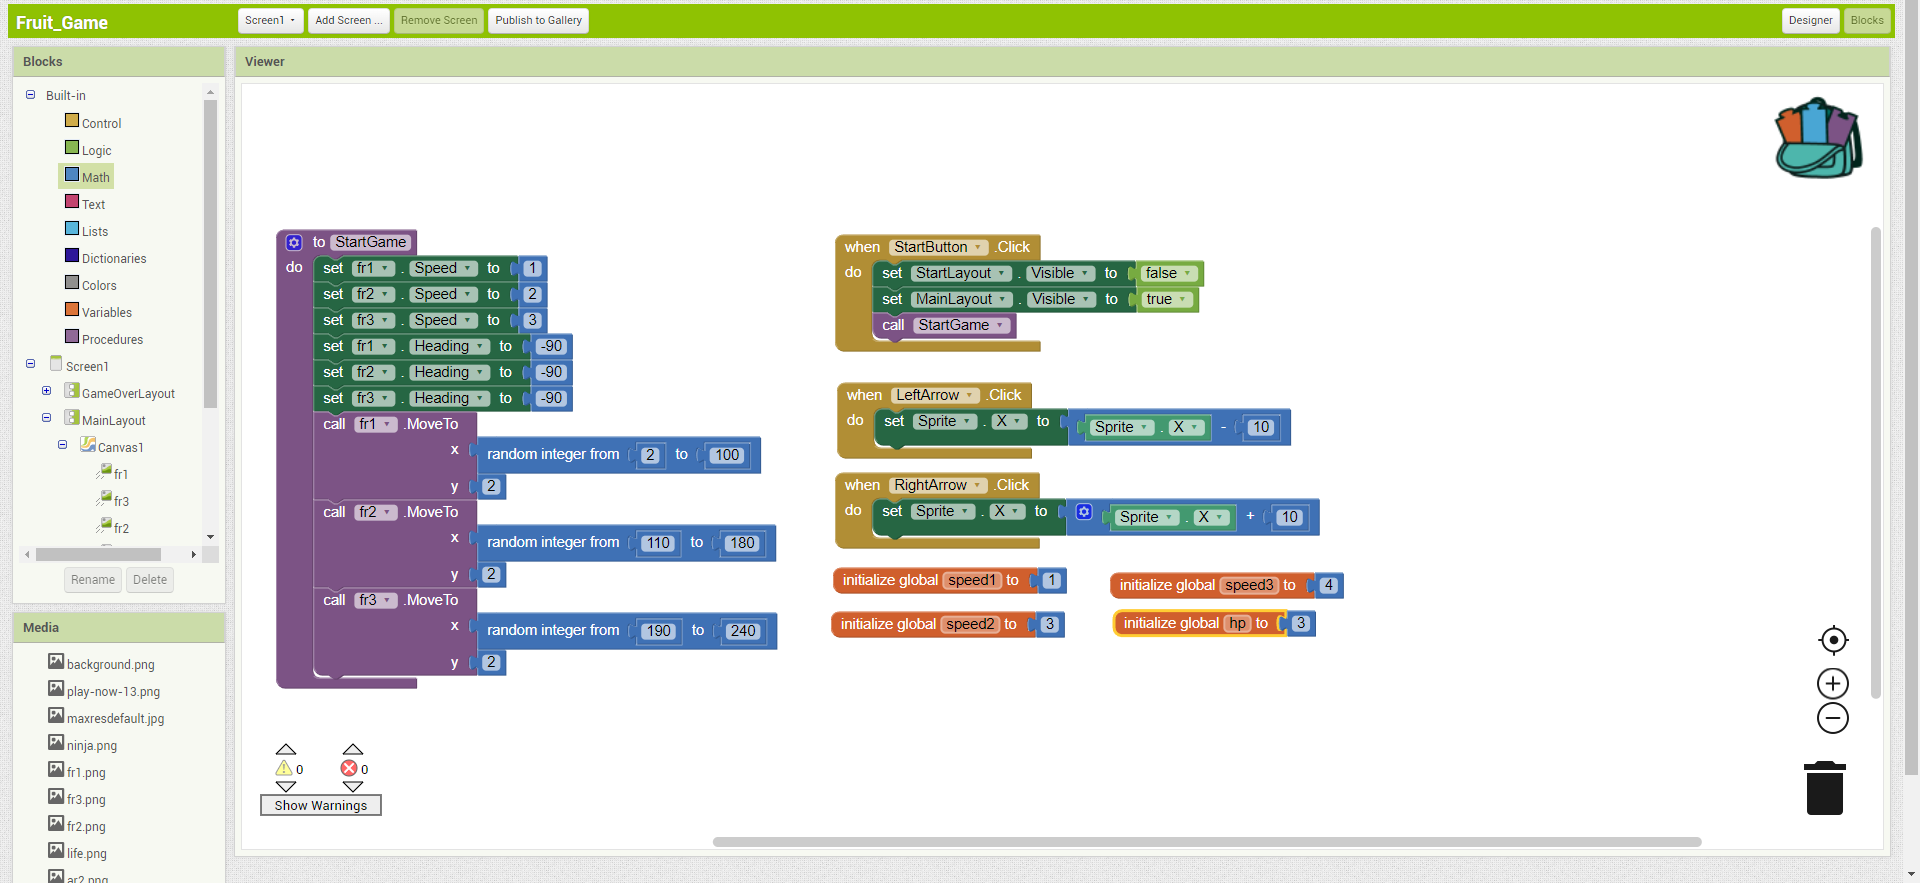
\includegraphics[width=1.0\linewidth,height=0.5\linewidth]{fig120019.png}
  \caption{Добавяне на променливи към играта}
\label{fig120019}
\end{figure}

Когато играчът докосне плод следва точките му да се увеличат. За тази цел отново ще се конструира процедура, тъй като и за трите плода трябва да се извика инструкцията, която променя точките.

\begin{figure}[H]
  \centering
  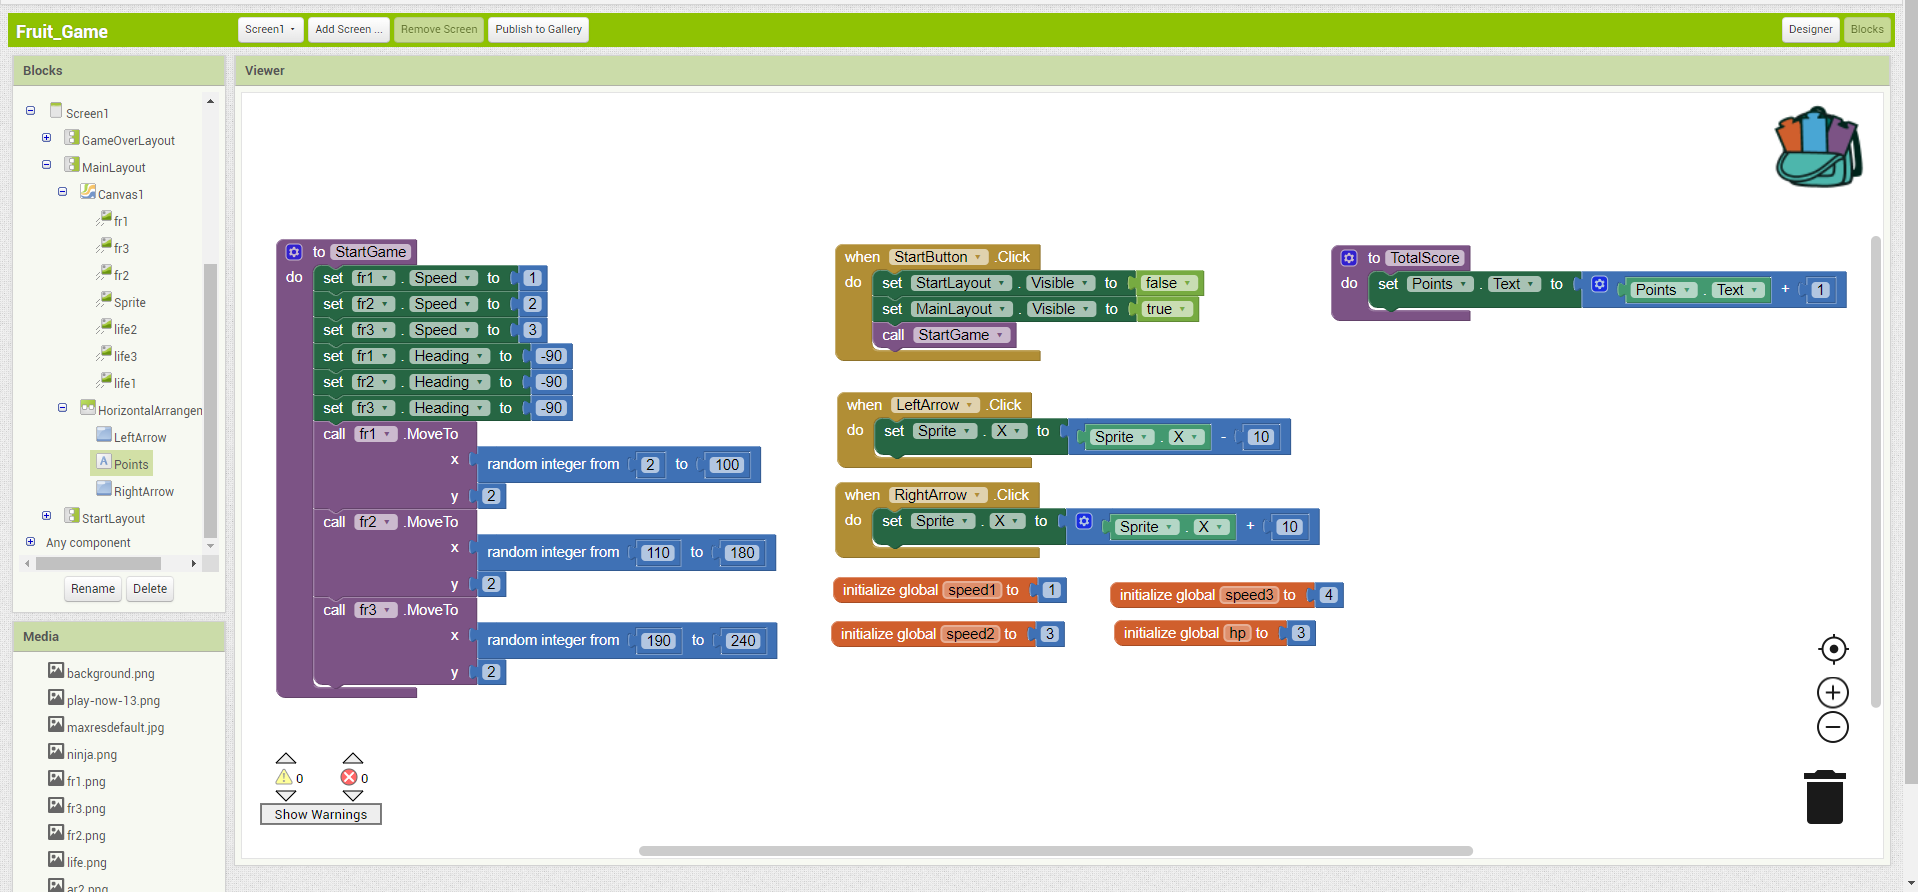
\includegraphics[width=1.0\linewidth,height=0.5\linewidth]{fig120020.png}
  \caption{Процедура за промяна на точките}
\label{fig120020}
\end{figure}

В следващата стъпка ще се добавят инструкции, които ще се изпълнят, когато играчът докосне плод. Алгоритъмът е следния - сменя се позицията на плода, увеличават се точките с 1 (има създадена процедура) и се увеличава скоростта на героя.

\begin{figure}[H]
  \centering
  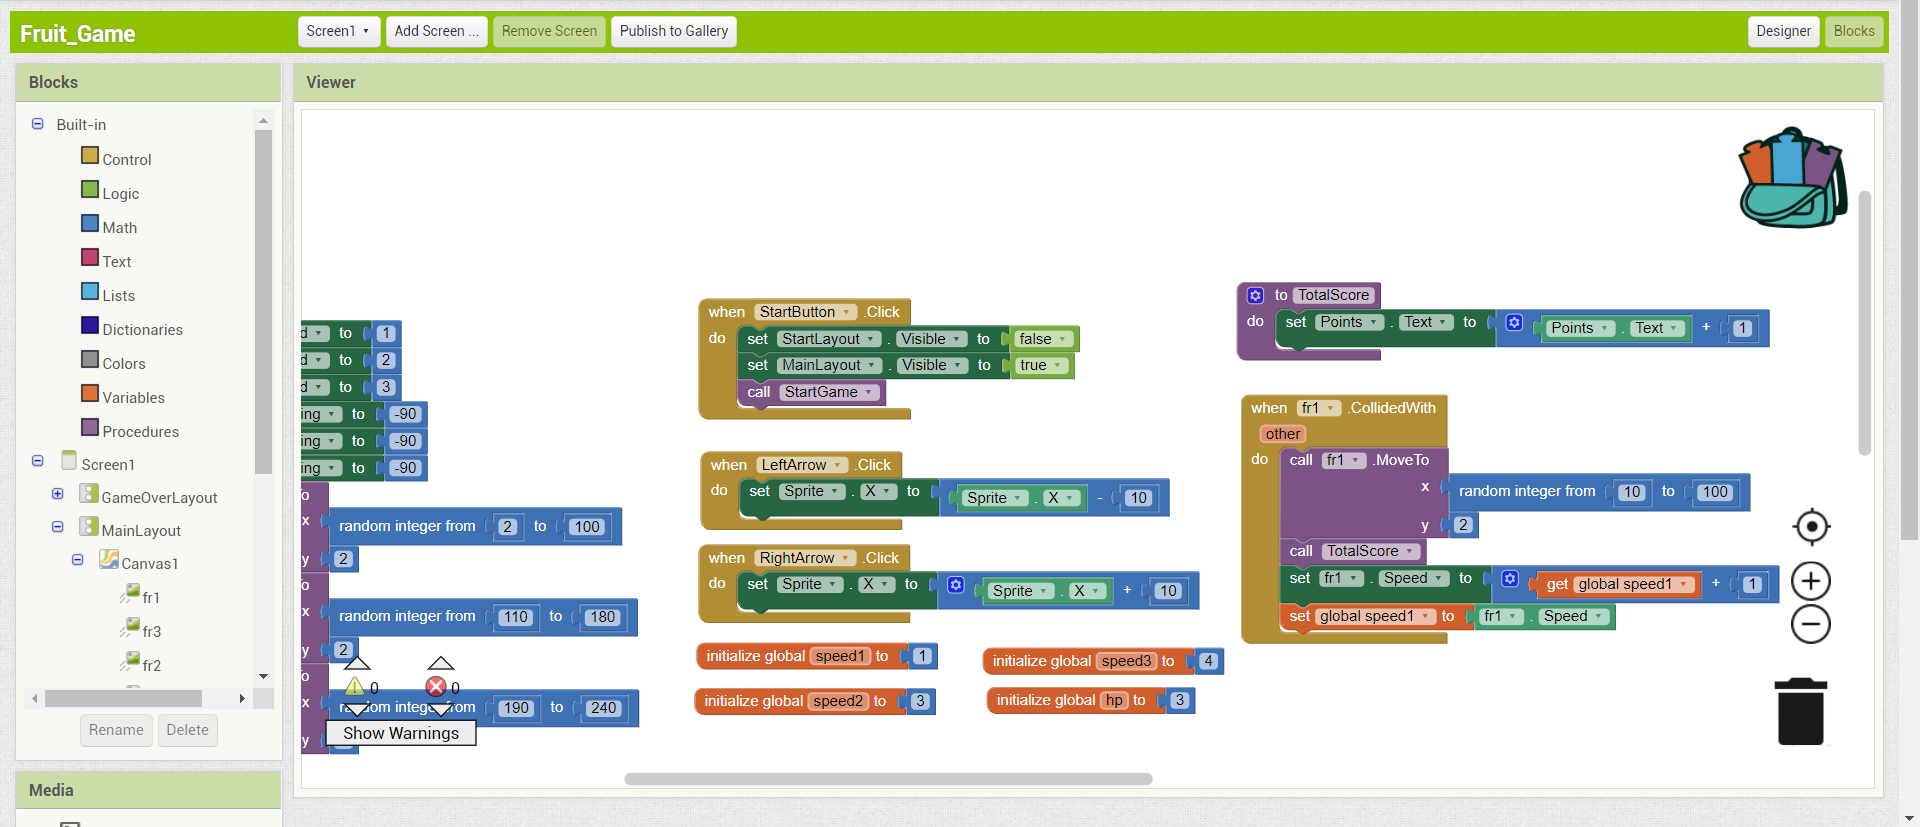
\includegraphics[width=1.0\linewidth,height=0.5\linewidth]{fig120021.png}
  \caption{Алгоритъм когато играчът докосне плод}
\label{fig120021}
\end{figure}

Този алгоритъм трябва да се конструира и за останалите герои плодове.

\begin{figure}[H]
  \centering
  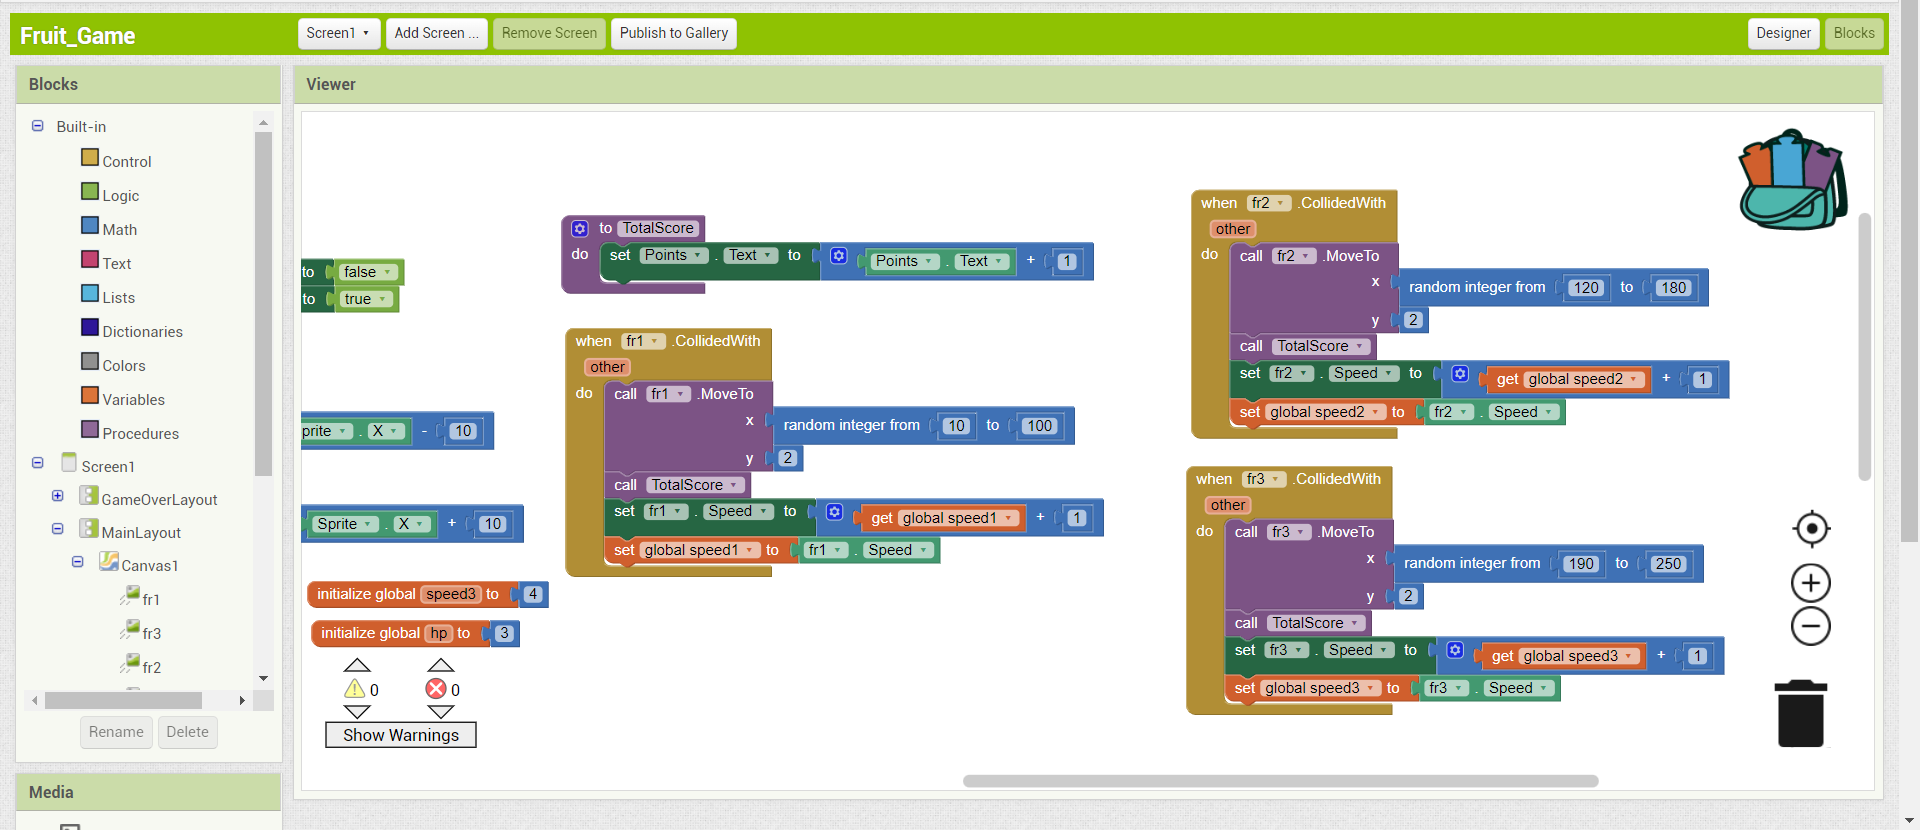
\includegraphics[width=1.0\linewidth,height=0.5\linewidth]{fig120022.png}
  \caption{Алгоритъмът за всички плодове}
\label{fig120022}
\end{figure}

Последната процедура, която трябва да се създаде е да се направи проверка дали играта трябва да приключи. Ако броя на животите е равен на 0, то тогава трябва да се скрие основния екран и да се появи екрана за край на играта. Също така скоростта на всички плодове трябва да стане равна на 0.

\begin{figure}[H]
  \centering
  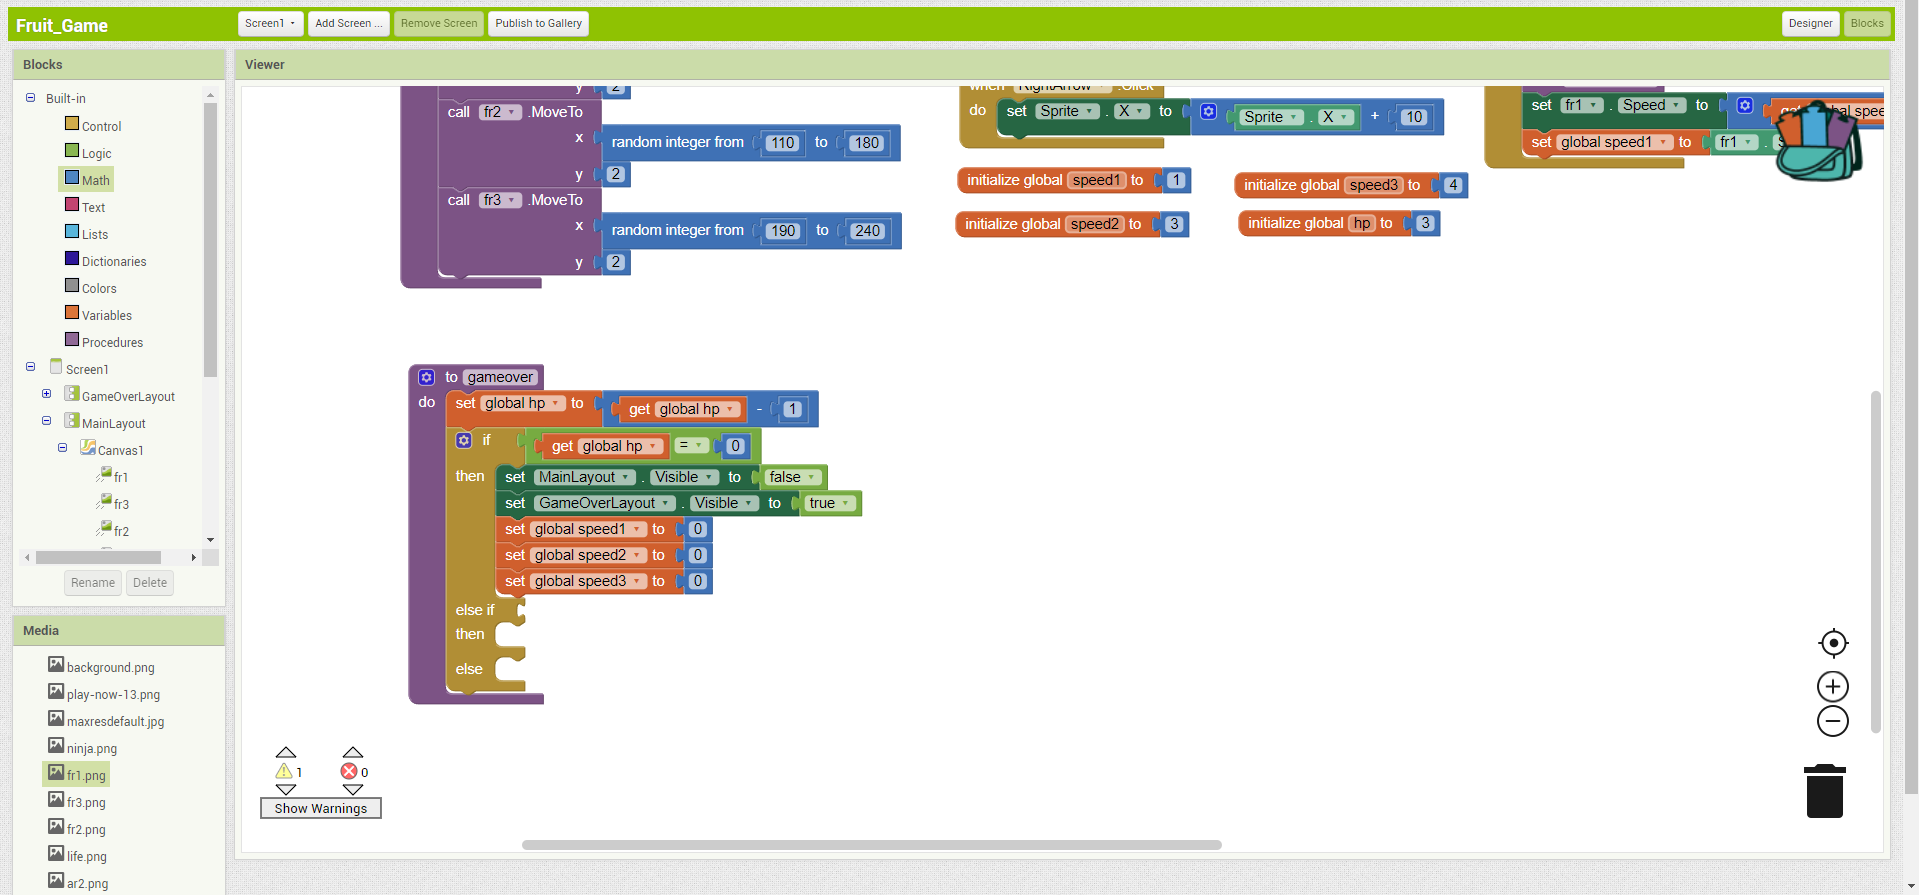
\includegraphics[width=1.0\linewidth,height=0.5\linewidth]{fig120023.png}
  \caption{Проверка дали героят губи играта}
\label{fig120023}
\end{figure}

Следва да се направят проверки ако животите са 2 или 1. Ако са два, това означава, че играчът е загубил 1 и трябва един от животите да се скрие. Отново трябва да се промени свойството Visible. Ако броят е 1, то това означава, че играчът е загубил 2 живота и следва да се скрие картинката и на още един от животите.

\begin{figure}[H]
  \centering
  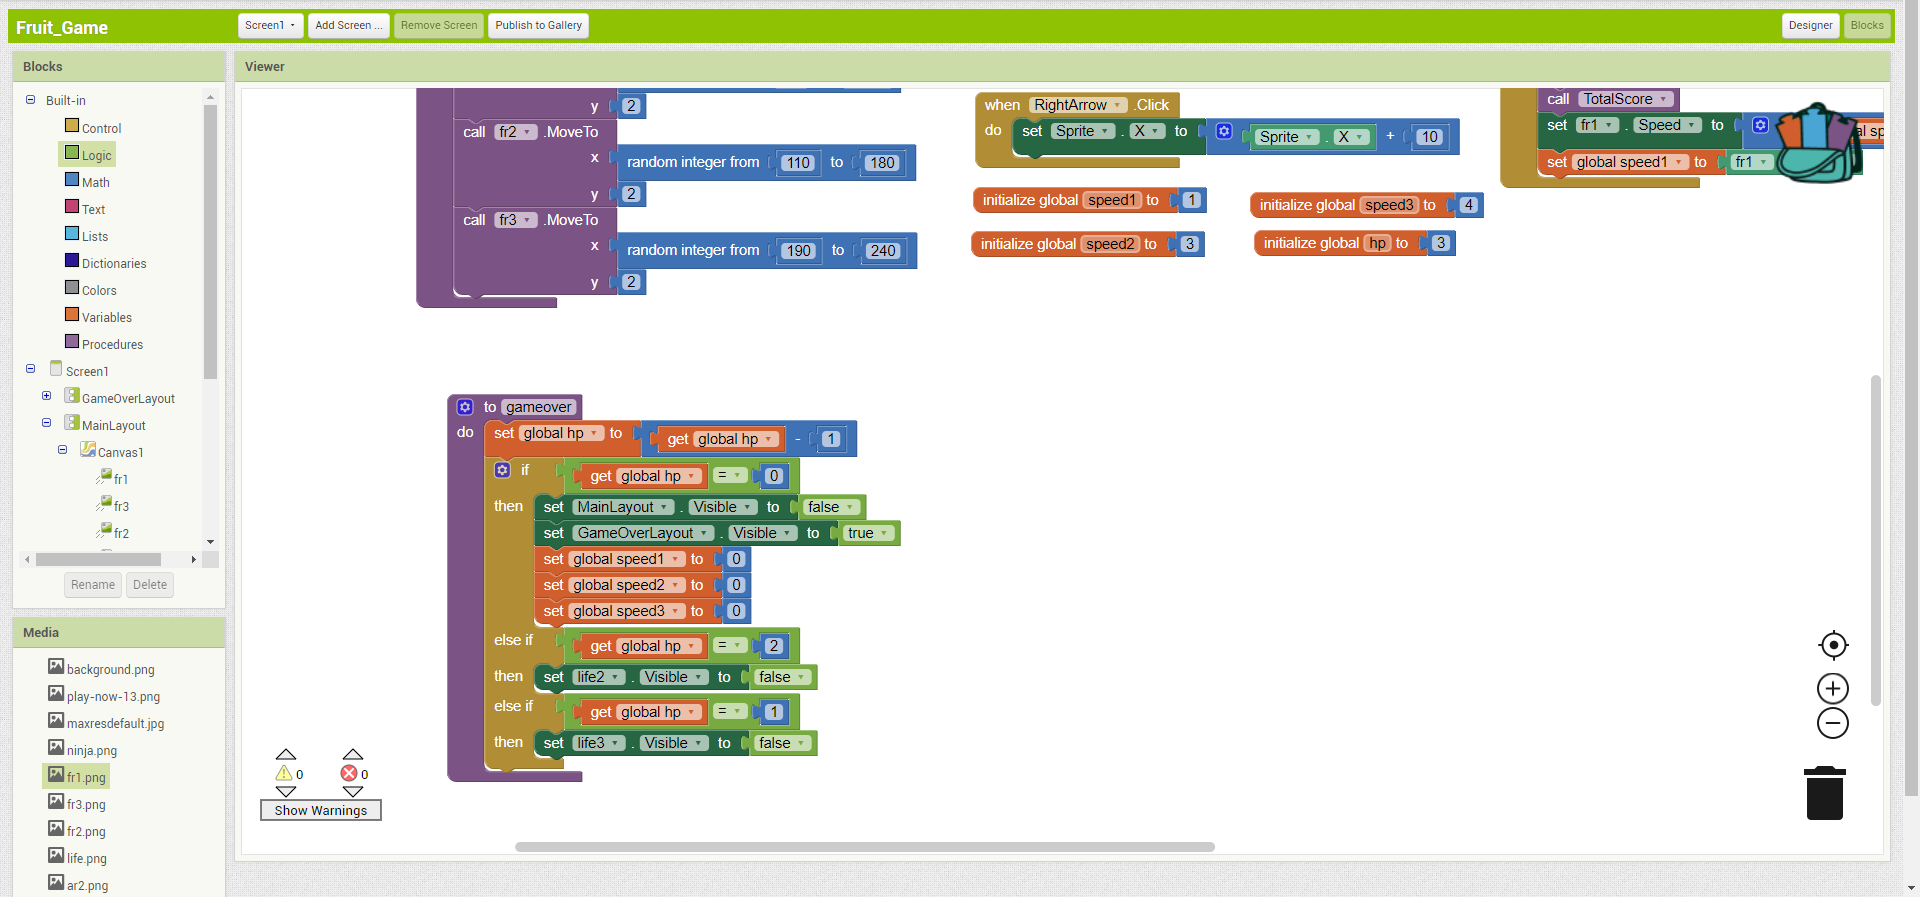
\includegraphics[width=1.0\linewidth,height=0.5\linewidth]{fig120024.png}
  \caption{Проверка дали героят има живот}
\label{fig120024}
\end{figure}

Когато героят плод докосне края на екрана, тогава трябва да се извика процедурата, за проверка за край на играта и да промени позицията си.

\begin{figure}[H]
  \centering
  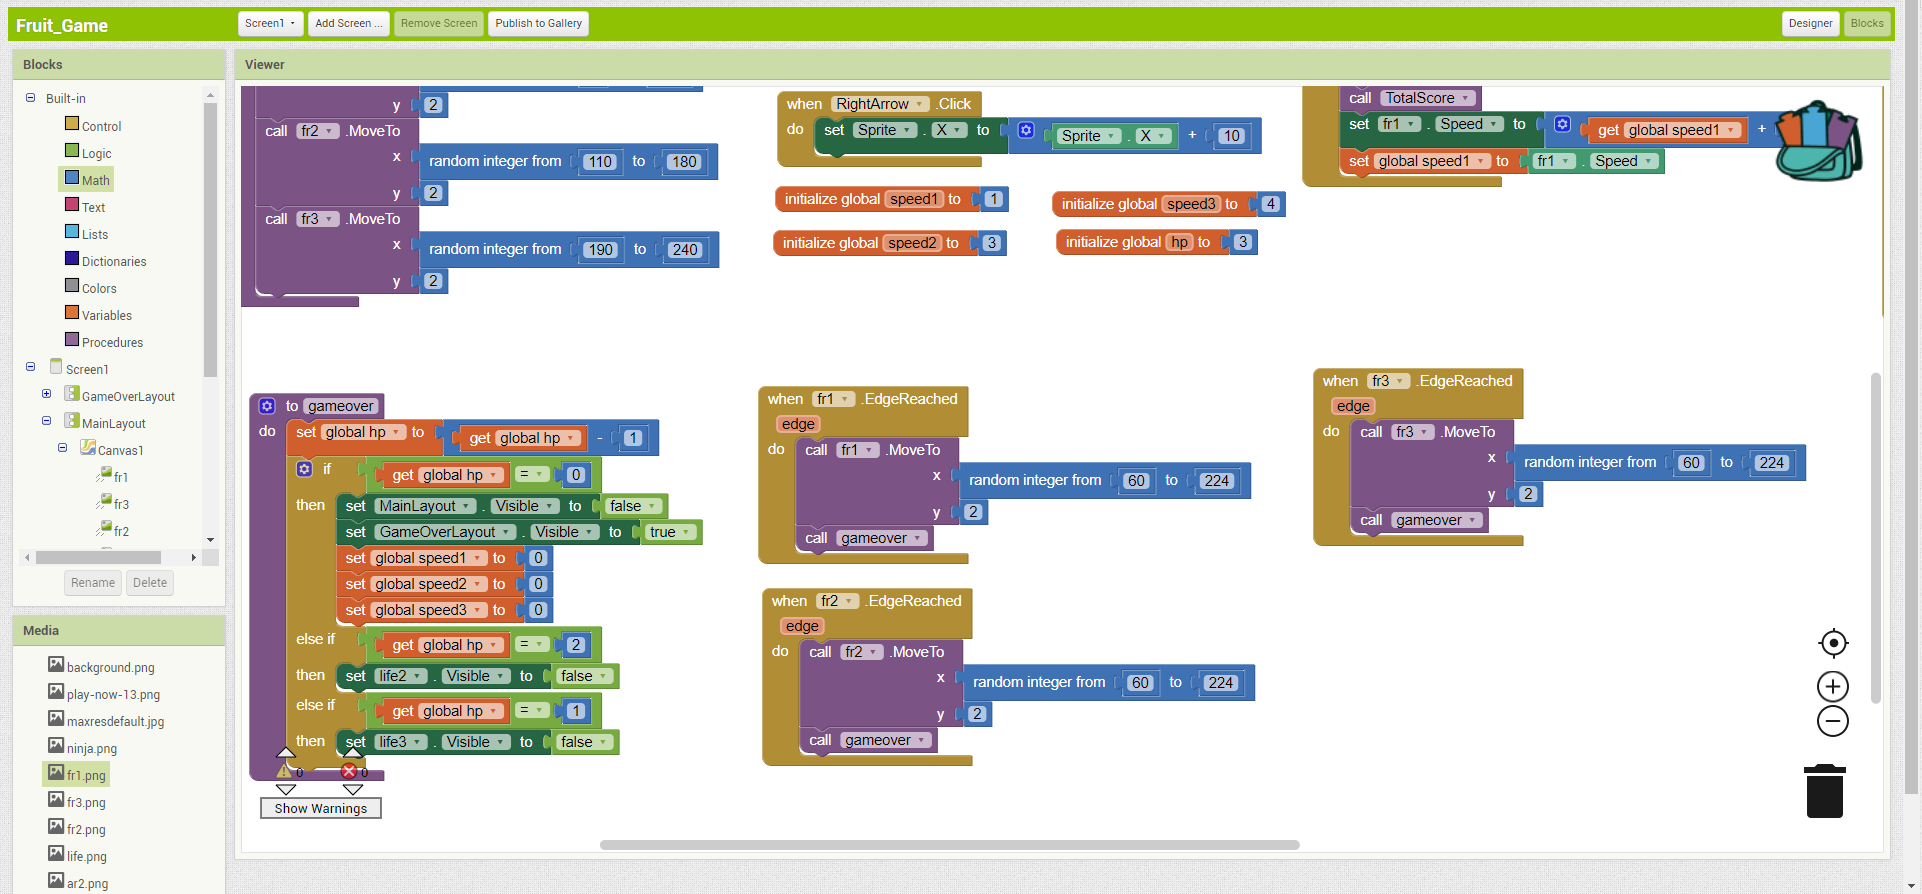
\includegraphics[width=1.0\linewidth,height=0.5\linewidth]{fig120025.png}
  \caption{Проверка дали плод е докоснал ръба}
\label{fig120025}
\end{figure}

Последните инструкции, които трябва да се конструират са, когато играта е приключила и играчът натисне бутона за рестартиране на играта.

\begin{figure}[H]
  \centering
  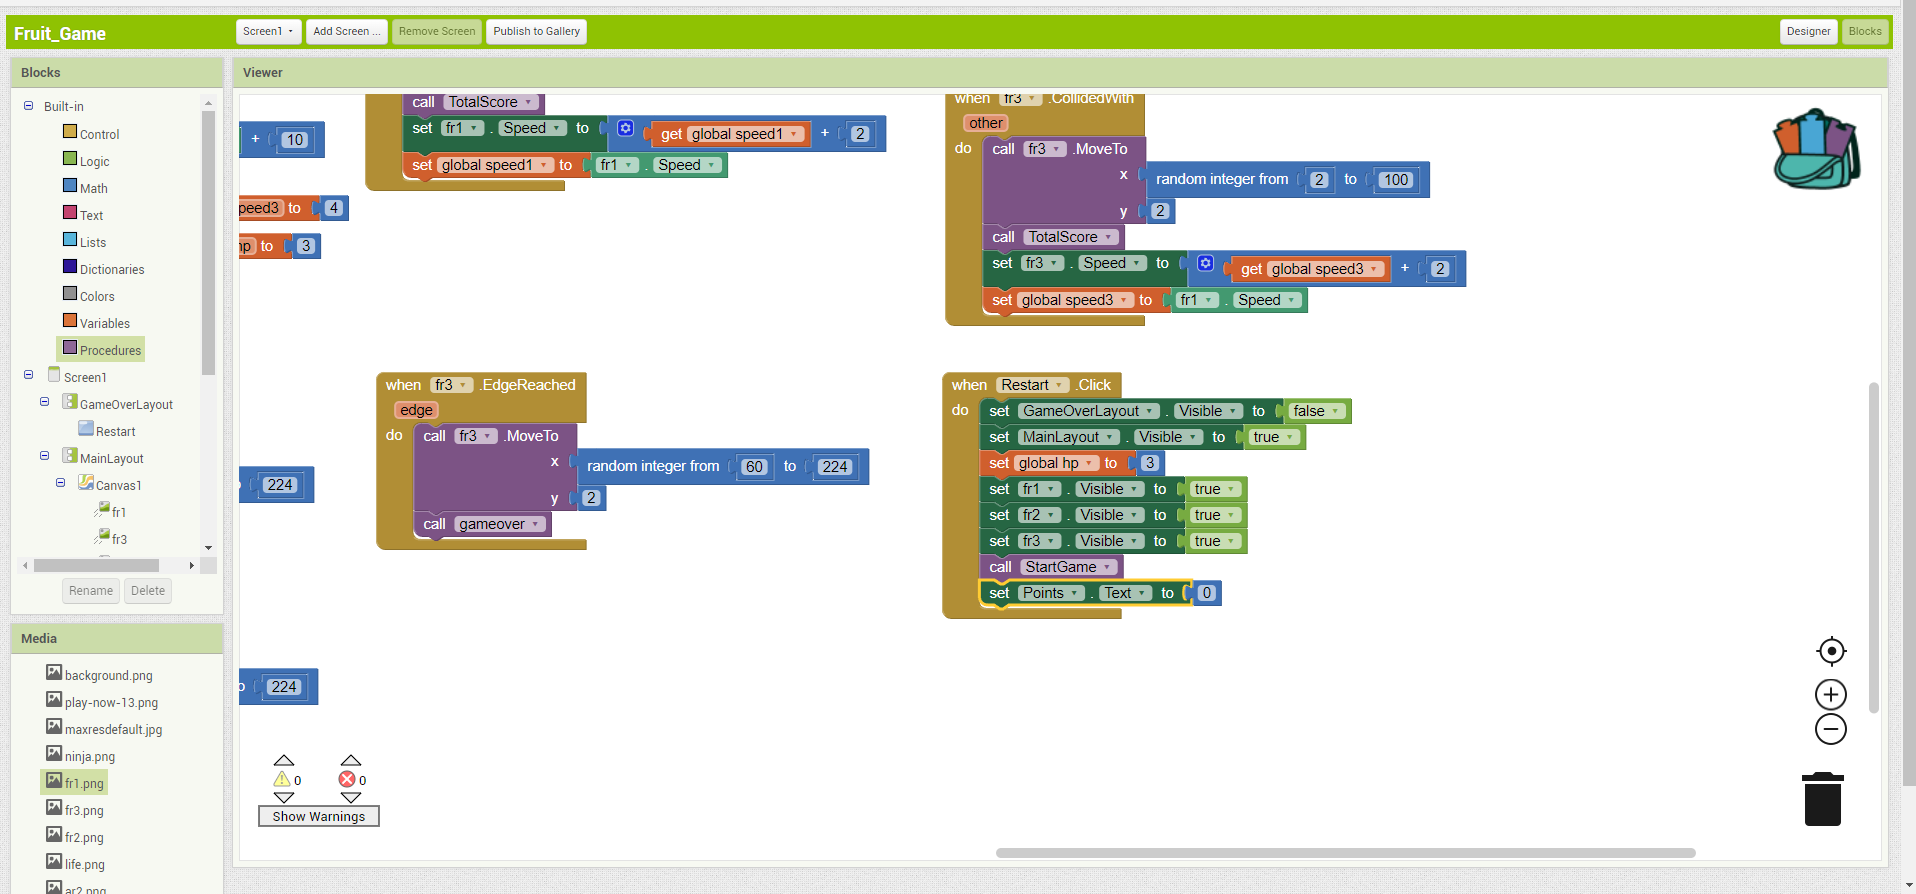
\includegraphics[width=1.0\linewidth,height=0.5\linewidth]{fig120026.png}
  \caption{Завършване на играта}
\label{fig120026}
\end{figure}

Играта е завършена. Следва да се тества върху телефона.
